% Options for packages loaded elsewhere
% Options for packages loaded elsewhere
\PassOptionsToPackage{unicode}{hyperref}
\PassOptionsToPackage{hyphens}{url}
\PassOptionsToPackage{dvipsnames,svgnames,x11names}{xcolor}
%
\documentclass[
  spanish,
  letterpaper,
  DIV=11,
  numbers=noendperiod]{scrartcl}
\usepackage{xcolor}
\usepackage[top=2.5cm,bottom=2.5cm,left=3cm,right=3cm]{geometry}
\usepackage{amsmath,amssymb}
\setcounter{secnumdepth}{5}
\usepackage{iftex}
\ifPDFTeX
  \usepackage[T1]{fontenc}
  \usepackage[utf8]{inputenc}
  \usepackage{textcomp} % provide euro and other symbols
\else % if luatex or xetex
  \usepackage{unicode-math} % this also loads fontspec
  \defaultfontfeatures{Scale=MatchLowercase}
  \defaultfontfeatures[\rmfamily]{Ligatures=TeX,Scale=1}
\fi
\usepackage{lmodern}
\ifPDFTeX\else
  % xetex/luatex font selection
\fi
% Use upquote if available, for straight quotes in verbatim environments
\IfFileExists{upquote.sty}{\usepackage{upquote}}{}
\IfFileExists{microtype.sty}{% use microtype if available
  \usepackage[]{microtype}
  \UseMicrotypeSet[protrusion]{basicmath} % disable protrusion for tt fonts
}{}
\makeatletter
\@ifundefined{KOMAClassName}{% if non-KOMA class
  \IfFileExists{parskip.sty}{%
    \usepackage{parskip}
  }{% else
    \setlength{\parindent}{0pt}
    \setlength{\parskip}{6pt plus 2pt minus 1pt}}
}{% if KOMA class
  \KOMAoptions{parskip=half}}
\makeatother
% Make \paragraph and \subparagraph free-standing
\makeatletter
\ifx\paragraph\undefined\else
  \let\oldparagraph\paragraph
  \renewcommand{\paragraph}{
    \@ifstar
      \xxxParagraphStar
      \xxxParagraphNoStar
  }
  \newcommand{\xxxParagraphStar}[1]{\oldparagraph*{#1}\mbox{}}
  \newcommand{\xxxParagraphNoStar}[1]{\oldparagraph{#1}\mbox{}}
\fi
\ifx\subparagraph\undefined\else
  \let\oldsubparagraph\subparagraph
  \renewcommand{\subparagraph}{
    \@ifstar
      \xxxSubParagraphStar
      \xxxSubParagraphNoStar
  }
  \newcommand{\xxxSubParagraphStar}[1]{\oldsubparagraph*{#1}\mbox{}}
  \newcommand{\xxxSubParagraphNoStar}[1]{\oldsubparagraph{#1}\mbox{}}
\fi
\makeatother

\usepackage{color}
\usepackage{fancyvrb}
\newcommand{\VerbBar}{|}
\newcommand{\VERB}{\Verb[commandchars=\\\{\}]}
\DefineVerbatimEnvironment{Highlighting}{Verbatim}{commandchars=\\\{\}}
% Add ',fontsize=\small' for more characters per line
\usepackage{framed}
\definecolor{shadecolor}{RGB}{241,243,245}
\newenvironment{Shaded}{\begin{snugshade}}{\end{snugshade}}
\newcommand{\AlertTok}[1]{\textcolor[rgb]{0.68,0.00,0.00}{#1}}
\newcommand{\AnnotationTok}[1]{\textcolor[rgb]{0.37,0.37,0.37}{#1}}
\newcommand{\AttributeTok}[1]{\textcolor[rgb]{0.40,0.45,0.13}{#1}}
\newcommand{\BaseNTok}[1]{\textcolor[rgb]{0.68,0.00,0.00}{#1}}
\newcommand{\BuiltInTok}[1]{\textcolor[rgb]{0.00,0.23,0.31}{#1}}
\newcommand{\CharTok}[1]{\textcolor[rgb]{0.13,0.47,0.30}{#1}}
\newcommand{\CommentTok}[1]{\textcolor[rgb]{0.37,0.37,0.37}{#1}}
\newcommand{\CommentVarTok}[1]{\textcolor[rgb]{0.37,0.37,0.37}{\textit{#1}}}
\newcommand{\ConstantTok}[1]{\textcolor[rgb]{0.56,0.35,0.01}{#1}}
\newcommand{\ControlFlowTok}[1]{\textcolor[rgb]{0.00,0.23,0.31}{\textbf{#1}}}
\newcommand{\DataTypeTok}[1]{\textcolor[rgb]{0.68,0.00,0.00}{#1}}
\newcommand{\DecValTok}[1]{\textcolor[rgb]{0.68,0.00,0.00}{#1}}
\newcommand{\DocumentationTok}[1]{\textcolor[rgb]{0.37,0.37,0.37}{\textit{#1}}}
\newcommand{\ErrorTok}[1]{\textcolor[rgb]{0.68,0.00,0.00}{#1}}
\newcommand{\ExtensionTok}[1]{\textcolor[rgb]{0.00,0.23,0.31}{#1}}
\newcommand{\FloatTok}[1]{\textcolor[rgb]{0.68,0.00,0.00}{#1}}
\newcommand{\FunctionTok}[1]{\textcolor[rgb]{0.28,0.35,0.67}{#1}}
\newcommand{\ImportTok}[1]{\textcolor[rgb]{0.00,0.46,0.62}{#1}}
\newcommand{\InformationTok}[1]{\textcolor[rgb]{0.37,0.37,0.37}{#1}}
\newcommand{\KeywordTok}[1]{\textcolor[rgb]{0.00,0.23,0.31}{\textbf{#1}}}
\newcommand{\NormalTok}[1]{\textcolor[rgb]{0.00,0.23,0.31}{#1}}
\newcommand{\OperatorTok}[1]{\textcolor[rgb]{0.37,0.37,0.37}{#1}}
\newcommand{\OtherTok}[1]{\textcolor[rgb]{0.00,0.23,0.31}{#1}}
\newcommand{\PreprocessorTok}[1]{\textcolor[rgb]{0.68,0.00,0.00}{#1}}
\newcommand{\RegionMarkerTok}[1]{\textcolor[rgb]{0.00,0.23,0.31}{#1}}
\newcommand{\SpecialCharTok}[1]{\textcolor[rgb]{0.37,0.37,0.37}{#1}}
\newcommand{\SpecialStringTok}[1]{\textcolor[rgb]{0.13,0.47,0.30}{#1}}
\newcommand{\StringTok}[1]{\textcolor[rgb]{0.13,0.47,0.30}{#1}}
\newcommand{\VariableTok}[1]{\textcolor[rgb]{0.07,0.07,0.07}{#1}}
\newcommand{\VerbatimStringTok}[1]{\textcolor[rgb]{0.13,0.47,0.30}{#1}}
\newcommand{\WarningTok}[1]{\textcolor[rgb]{0.37,0.37,0.37}{\textit{#1}}}

\usepackage{longtable,booktabs,array}
\newcounter{none} % for unnumbered tables
\usepackage{calc} % for calculating minipage widths
% Correct order of tables after \paragraph or \subparagraph
\usepackage{etoolbox}
\makeatletter
\patchcmd\longtable{\par}{\if@noskipsec\mbox{}\fi\par}{}{}
\makeatother
% Allow footnotes in longtable head/foot
\IfFileExists{footnotehyper.sty}{\usepackage{footnotehyper}}{\usepackage{footnote}}
\makesavenoteenv{longtable}
\usepackage{graphicx}
\makeatletter
\newsavebox\pandoc@box
\newcommand*\pandocbounded[1]{% scales image to fit in text height/width
  \sbox\pandoc@box{#1}%
  \Gscale@div\@tempa{\textheight}{\dimexpr\ht\pandoc@box+\dp\pandoc@box\relax}%
  \Gscale@div\@tempb{\linewidth}{\wd\pandoc@box}%
  \ifdim\@tempb\p@<\@tempa\p@\let\@tempa\@tempb\fi% select the smaller of both
  \ifdim\@tempa\p@<\p@\scalebox{\@tempa}{\usebox\pandoc@box}%
  \else\usebox{\pandoc@box}%
  \fi%
}
% Set default figure placement to htbp
\def\fps@figure{htbp}
\makeatother



\ifLuaTeX
\usepackage[bidi=basic,shorthands=off]{babel}
\else
\usepackage[bidi=default,shorthands=off]{babel}
\fi
\ifLuaTeX
  \usepackage{selnolig} % disable illegal ligatures
\fi


\setlength{\emergencystretch}{3em} % prevent overfull lines

\providecommand{\tightlist}{%
  \setlength{\itemsep}{0pt}\setlength{\parskip}{0pt}}



 


\usepackage{booktabs}
\usepackage{longtable}
\usepackage{array}
\usepackage{multirow}
\usepackage{wrapfig}
\usepackage{float}
\usepackage{colortbl}
\usepackage{pdflscape}
\usepackage{tabu}
\usepackage{threeparttable}
\usepackage{threeparttablex}
\usepackage[normalem]{ulem}
\usepackage{makecell}
\usepackage{xcolor}
\usepackage{scrlayer-scrpage}
\usepackage{float}
\floatplacement{figure}{H}
\floatplacement{table}{H}
\pagestyle{scrheadings}
\ihead{\bfseries Proyecto RLM -- Entrega 1}
\setkomafont{pageheadfoot}{\normalfont\small}
\KOMAoptions{headsepline=true}
\KOMAoption{captions}{tableheading}
\makeatletter
\@ifpackageloaded{caption}{}{\usepackage{caption}}
\AtBeginDocument{%
\ifdefined\contentsname
  \renewcommand*\contentsname{Tabla de contenidos}
\else
  \newcommand\contentsname{Tabla de contenidos}
\fi
\ifdefined\listfigurename
  \renewcommand*\listfigurename{Listado de Figuras}
\else
  \newcommand\listfigurename{Listado de Figuras}
\fi
\ifdefined\listtablename
  \renewcommand*\listtablename{Listado de Tablas}
\else
  \newcommand\listtablename{Listado de Tablas}
\fi
\ifdefined\figurename
  \renewcommand*\figurename{Figura}
\else
  \newcommand\figurename{Figura}
\fi
\ifdefined\tablename
  \renewcommand*\tablename{Tabla}
\else
  \newcommand\tablename{Tabla}
\fi
}
\@ifpackageloaded{float}{}{\usepackage{float}}
\floatstyle{ruled}
\@ifundefined{c@chapter}{\newfloat{codelisting}{h}{lop}}{\newfloat{codelisting}{h}{lop}[chapter]}
\floatname{codelisting}{Listado}
\newcommand*\listoflistings{\listof{codelisting}{Listado de Listados}}
\makeatother
\makeatletter
\makeatother
\makeatletter
\@ifpackageloaded{caption}{}{\usepackage{caption}}
\@ifpackageloaded{subcaption}{}{\usepackage{subcaption}}
\makeatother
\usepackage{bookmark}
\IfFileExists{xurl.sty}{\usepackage{xurl}}{} % add URL line breaks if available
\urlstyle{same}
\hypersetup{
  pdflang={es},
  colorlinks=true,
  linkcolor={black},
  filecolor={Maroon},
  citecolor={black},
  urlcolor={black},
  pdfcreator={LaTeX via pandoc}}


\author{}
\date{}
\begin{document}


\begin{titlepage}
\centering

\includegraphics[width=10cm]{bandera-01.jpg}\\[0.2cm]

{\Large \textbf{Universidad Nacional de Colombia}}\\[0.15cm]
{\normalsize Departamento de Estadística -- Facultad de Ciencias}\\[2cm]

{\normalsize Análisis de Regresión – 3006918}\\[2cm]

{\bfseries MODELADO DE LOS INGRESOS MENSUALES DE EMPLEADOS EN COLOMBIA}\\[0.15cm]
{\small Aplicación de un Modelo de Regresión Lineal Múltiple}\\[2cm]

{\small Docente: Isabel Cristina Ramírez Guevara}\\[2cm]

{\small Yuliany Cifuentes Rondon}\\
{\small Daniela Cataño Hernández}\\
{\small Samir Alejandro Centeno Torrado}\\[2cm]

\vfill
{\small Medellín, Colombia \quad -- \quad Semestre 2026-1}

\end{titlepage}
\thispagestyle{empty}

\newpage
\renewcommand*\contentsname{}
\begin{center}
{\Large\bfseries Índice}
\end{center}
\vspace{0.5cm}
\tableofcontents
\newpage

\section{Enunciado del proyecto}\label{enunciado-del-proyecto}

El proyecto consiste en buscar una base de datos con datos colombianos
que contenga una variable de respuesta continua (𝑌), al menos cinco
covariables continuas (𝑋) y una variable categórica (𝑍) con al menos
tres categorías. Los análisis se realizan con máximo 100 registros. El
proyecto tiene tres entregas y una exposición final.

\begin{enumerate}
\def\labelenumi{\arabic{enumi}.}
\item
  Contextualizar el fenómeno a modelar: explicar el significado de la
  variable de respuesta y las covariables, la relevancia del estudio y
  su objetivo. Establecer dos hipótesis que se desean probar con el
  modelo.
\item
  Realizar un análisis descriptivo exhaustivo y pertinente para el tipo
  de modelo que se va a aplicar.
\end{enumerate}

\section{Introducción}\label{introducciuxf3n}

El ingreso laboral es uno de los principales determinantes del bienestar
de los hogares colombianos y uno de los indicadores más utilizados para
analizar la desigualdad económica del país. Explicar por qué unos
trabajadores ganan más que otros es una pregunta central de la economía
laboral, y la respuesta habitual ---propuesta por Mincer (1974)--- es
que el ingreso depende principalmente de la acumulación de capital
humano (educación y experiencia), de la intensidad con que se trabaja
(horas) y de las características del empleo (tipo de vinculación y
sector económico).

En Colombia, donde la informalidad laboral y la heterogeneidad sectorial
son altas, estos factores no siempre se traducen en el mismo nivel de
ingreso: dos personas con la misma escolaridad pueden percibir
remuneraciones muy distintas según su posición ocupacional o la rama de
actividad en la que trabajan. Este proyecto busca cuantificar, a partir
de microdatos de la Gran Encuesta Integrada de Hogares (GEIH), qué tanto
explican estas variables la variabilidad del ingreso laboral mensual.

\section{Contextualización del problema}

El ingreso laboral es una de las variables centrales para el estudio del bienestar
economico y del funcionamiento del mercado de trabajo. Desde la teoria del capital
humano, propuesta originalmente por Mincer, se plantea que el salario de un
individuo puede explicarse en buena medida por su nivel de escolaridad y por su
experiencia laboral entendida esta ultima como una proxy del entrenamiento
adquirido en el puesto de trabajo \cite{mincer1974}. Este marco teorico dio origen
a la conocida \emph{ecuación de Mincer}, que modela el logaritmo del ingreso como
funcion lineal de la educación y de la experiencia (y su forma cuadratica) y que
constituye hasta hoy el punto de partida estandar para el analisis empirico de los
determinantes salariales.

En el caso colombiano, esta relacion ha sido documentada de manera consistente.
Núñez y Sánchez \cite{nunez1998} utilizando informacion de encuestas de hogares
del DANE encuentran que la escolaridad ha sido el factor con mayor poder
explicativo sobre los diferenciales de ingreso laboral en el pais, y que su efecto
se ha mantenido estable a lo largo de distintos periodos. En la misma linea
Guataquí et al. \cite{guataqui}, con datos de la Gran Encuesta Integrada de
Hogares (GEIH), muestran que ademas de la educacion, variables como la posicion
ocupacional y la experiencia potencial explican una parte relevante de la
heterogeneidad salarial observada, y advierten sobre la importancia de separar
estos efectos entre asalariados y trabajadores por cuenta propia, dado que ambos
grupos responden a estructuras de determinacion de ingresos distintas.

Estudios mas recientes del banco de la republica \cite{banrep2021} confirman que
estos patrones persisten e incluso se intensifican en contextos de choques
economicos: al modelar los determinantes del ingreso laboral para el periodo
2010-2019, encuentran que la brecha salarial asociada al sexo del trabajador y a
la posicion ocupacional continua siendo estadisticamente significativa una vez
controlado por nivel educativo. A nivel de subgrupos poblacionales especificos,
Panorama Económico \cite{panorama2019} aplica una ecuación minceriana a
profesionales en economia y encuentra que un año adicional de formacion escolar
incrementa significativamente la probabilidad de percibir ingresos mas altos,
evidenciando que el efecto de la educacion sobre el salario no es homogeneo entre
grupos ocupacionales, sino que varia segun el perfil profesional analizado.

En conjunto, esta literatura sugiere que un modelo del ingreso laboral en Colombia
debe incorporar, como minimo, variables asociadas a la educacion, la experiencia o
antigüedad laboral y la heterogeneidad sectorial del mercado de trabajo, dado que
son los determinantes que de manera recurrente resultan significativos en los
estudios previos. El presente proyecto retoma este marco para proponer un modelo
de regresión lineal multiple sobre una muestra de trabajadores colombianos,
incorporando la escolaridad, la edad (y su termino cuadratico), la antigüedad en
el empleo actual y la intensidad de trabajo (horas semanales) como covariables
continuas, y la rama de actividad económica como variable categorica, con el fin
de evaluar el peso relativo de estos factores sobre el ingreso laboral.

\section{Objetivo general}

Desarrollar un modelo de regresión lineal multiple que permita explicar el
logaritmo del ingreso laboral mensual de los trabajadores en Colombia a partir de
variables asociadas a la teoria del capital humano y a la literatura empirica
sobre determinantes salariales en el pais, especificamente las horas de trabajo
semanales, la escolaridad, la edad, la antigüedad en el empleo actual y la rama
de actividad económica en la que se desempeña el trabajador.

\section{Relevancia del estudio}

La identificacion de los factores que determinan los ingresos laborales es un
tema central en la economia laboral y ha sido ampliamente estudiado en Colombia
desde la perspectiva del capital humano \cite{mincer1974, nunez1998}. Sin embargo,
buena parte de esta literatura se ha concentrado en variables de escolaridad y
experiencia, dejando en un segundo plano el análisis conjunto con variables como
la intensidad y continuidad laboral (horas trabajadas y antigüedad en el empleo
actual). Este proyecto busca aportar evidencia adicional sobre el peso
relativo de estos factores frente a los determinantes tradicionales, replicando
ademas la evidencia existente sobre las diferencias de ingreso asociadas a la
rama de actividad económica documentadas por el banco de la republica \cite{banrep2021}.
Los resultados permitiran establecer que características tienen una influencia
significativa sobre los salarios en la muestra analizada y contrastar estos
hallazgos con lo reportado en la literatura previa.

\subsection{Variables seleccionadas}\label{variables-seleccionadas}

\begingroup\fontsize{8}{10}\selectfont

\begin{longtable}[t]{>{\raggedright\arraybackslash}p{3.3cm}>{\raggedright\arraybackslash}p{3cm}>{\centering\arraybackslash}p{1cm}>{\centering\arraybackslash}p{1.8cm}>{\raggedright\arraybackslash}p{5.3cm}}
\caption{\label{tab:tabla-variables}Variables seleccionadas, rol en el modelo y significado en el estudio.}\\
\toprule
Nombre & Código & Rol & Tipo & Significado\\
\midrule
\endfirsthead
\caption[]{Variables seleccionadas, rol en el modelo y significado en el estudio. \textit{(continued)}}\\
\toprule
Nombre & Código & Rol & Tipo & Significado\\
\midrule
\endhead

\endfoot
\bottomrule
\endlastfoot
Logaritmo del ingreso laboral mensual & INGLABO (transformada) & Y & Continua & Ingreso laboral mensual transformado a escala logarítmica para reducir la asimetría de la distribución.\\
Horas trabajadas por semana & P6800 & X1 & Continua & Intensidad del trabajo desarrollado durante la semana de referencia.\\
Años de escolaridad & P3042 (recodificada) & X2 & Continua & Años de educación formal aprobados, recodificados a partir del nivel educativo alcanzado; mide la acumulación de capital humano.\\
Edad & P6040 & X3 & Continua & Edad de la persona en años cumplidos; aproxima el ciclo de vida laboral.\\
Edad al cuadrado & Derivada de X3 & X4 & Continua & Captura el efecto no lineal (rendimientos decrecientes) de la edad sobre el ingreso.\\
\addlinespace
Antigüedad en el empleo actual & P6426 & X5 & Continua & Meses en el empleo u ocupación actual; aproxima estabilidad y experiencia específica.\\
Rama de actividad económica & RAMA2D\_R4 & X6 (Z) & Categórica & Sector económico (CIIU, 2 dígitos) en el que se desempeña el trabajador.\\*
\end{longtable}
\endgroup{}

\subsubsection{Descripción detallada de las
variables}\label{descripciuxf3n-detallada-de-las-variables}

\textbf{Y: Logaritmo del ingreso laboral mensual.} La variable de
respuesta corresponde al ingreso laboral mensual percibido por las
personas ocupadas incluidas en la GEIH, expresado en pesos colombianos.
Dado que en economía laboral es ampliamente reconocido que la
distribución de los ingresos presenta una marcada asimetría positiva, la
variable dependiente se transforma mediante el logaritmo natural, lo que
reduce la asimetría, disminuye la influencia de valores extremos y
permite interpretar los coeficientes del modelo como variaciones
porcentuales aproximadas del ingreso (especificación clásica de Mincer,
1974).

\textbf{X1: Horas trabajadas por semana.} Número de horas que la persona
trabajó habitualmente durante la semana de referencia en su ocupación
principal. Se espera una relación positiva con el ingreso.

\textbf{X2: Años de escolaridad.} Construida a partir del nivel
educativo alcanzado (P3042), recodificando cada uno de los 13 niveles a
un número típico de años acumulados de educación formal. Para los
niveles hasta la educación media, los años corresponden a la duración
legal establecida por la Ley 115 de 1994 (primaria: 5 años; básica
secundaria: 4 años adicionales; media: 2 años adicionales). Para los
niveles de educación superior (técnica, tecnológica, universitaria y
posgrados), se asume la duración típica de cada programa, siguiendo la
convención de conversión utilizada en estudios de determinantes
salariales con la GEIH (Núñez \& Sánchez, 1998), dado que la encuesta no
permite distinguir la duración exacta cursada por cada persona dentro de
ese nivel.

\textbf{X3: Edad.} Edad de la persona en años cumplidos al momento de la
encuesta. Se utiliza como proxy del ciclo de vida laboral en lugar de la
experiencia potencial (Edad - Escolaridad - 6), evitando así que esta
covariable dependa de la variable de escolaridad ya construida, y
reduciendo el número de transformaciones y supuestos encadenados sobre
la base de datos.

\textbf{X4: Edad al cuadrado.} Incorpora la relación cóncava entre edad
e ingreso: los ingresos aumentan con la edad, pero a una tasa
decreciente, consistente con el perfil edad-ingreso documentado en la
literatura de capital humano.

\textbf{X5: Antigüedad en el empleo actual.} Meses que el trabajador
lleva en su empleo u ocupación actual; aproxima estabilidad laboral y
experiencia específica en la organización.

\textbf{X6 (Z): Rama de actividad económica.} Sector económico en el que
se desempeña el trabajador, agrupado según la Clasificación Industrial
Internacional Uniforme (CIIU) a 2 dígitos.

\section{Modelo matemático
propuesto}\label{modelo-matemuxe1tico-propuesto}

Con fundamento en la teoría del capital humano y en la especificación
clásica de la ecuación de ingresos de Mincer, se propone estimar un
modelo de regresión lineal múltiple en el que el logaritmo natural del
ingreso laboral mensual constituye la variable dependiente:

\[\ln(Y_i)=\beta_0+\beta_1X_{1i}+\beta_2X_{2i}
+\beta_3X_{3i}
+\beta_4X_{4i}
+\beta_5X_{5i}
+\beta_6X_{6i}
+\varepsilon_i\]

donde \(X_1\): horas trabajadas por semana; \(X_2\): años de
escolaridad; \(X_3\): edad; \(X_4\): edad al cuadrado; \(X_5\):
antigüedad en el empleo actual; \(X_6\): rama de actividad económica
(dummy); \(\beta_0\): intercepto; \(\varepsilon_i\): error aleatorio.

Antes de estimar el modelo definitivo se verificará el cumplimiento de
los supuestos de la regresión lineal múltiple, evaluando la existencia
de multicolinealidad mediante el Factor de Inflación de la Varianza
(VIF), la homocedasticidad de los residuos, la normalidad de los errores
y la posible presencia de observaciones influyentes (Montgomery et al.,
2021).

\subsection{Hipótesis}\label{hipuxf3tesis}

Las siguientes hipótesis se desprenden directamente de la
contextualización presentada en la Introducción y la Relevancia (teoría
del capital humano de Mincer, 1974, y la heterogeneidad del mercado
laboral colombiano). Cada una se plantea de forma que pueda traducirse,
en la etapa de modelación, en el signo y la significancia esperados de
parámetros específicos del modelo
\(\ln(Y_i)=\beta_0+\beta_1X_{1i}+\dots+\beta_6X_{6i}+\varepsilon_i\).

\textbf{Hipótesis 1: la escolaridad y la edad explican una parte
sustancial de la variabilidad del ingreso laboral.} De acuerdo con la
teoría del capital humano, se espera que los trabajadores con mayor
escolaridad perciban ingresos más altos, y que el ingreso siga un perfil
cóncavo respecto a la edad ---creciente en las primeras etapas de la
vida laboral, hasta el punto en que los rendimientos empiezan a
decrecer---. En términos del modelo, esta hipótesis se traduce en
\(\beta_2>0\) (escolaridad), \(\beta_3>0\) (edad) y \(\beta_4<0\) (edad
al cuadrado), reflejando el perfil cóncavo típico de la ecuación de
Mincer; se espera además que ambos coeficientes sean estadísticamente
significativos.

\textbf{Hipótesis 2: la rama de actividad económica genera diferencias
sistemáticas en el ingreso, incluso después de considerar la escolaridad
y la edad.} Dada la heterogeneidad e informalidad del mercado laboral
colombiano descrita en la Relevancia, se espera que existan brechas de
ingreso entre sectores económicos que la educación y la edad por sí
solas no logran explicar. En el modelo, esto se traduce en que al menos
algunos de los coeficientes asociados a las variables dummy de rama de
actividad (\(\beta_6\)) sean estadísticamente significativos y distintos
de cero.

\section{Análisis descriptivo}\label{anuxe1lisis-descriptivo}

\subsection{Información sobre la base de
datos}\label{informaciuxf3n-sobre-la-base-de-datos}

La base de datos utilizada corresponde a la Gran Encuesta Integrada de
Hogares (GEIH), operativo de enero de 2024, publicada por el
Departamento Administrativo Nacional de Estadística (DANE). Los
microdatos se descargaron en formato .zip desde el archivo nacional de
microdatos del DANE (operativo de enero), disponible en el catálogo
público:
\url{https://microdatos.dane.gov.co/index.php/catalog/819/data-dictionary}.
Se utilizan dos de sus módulos:

\begin{itemize}
\tightlist
\item
  \textbf{Ocupados}: contiene las variables laborales de las personas
  ocupadas (ingreso, horas trabajadas, antigüedad, rama de actividad,
  entre otras).
\item
  \textbf{Características generales, seguridad social en salud y
  educación}: contiene las variables demográficas y educativas (edad,
  nivel educativo, grado aprobado).
\end{itemize}

Ambos módulos se identifican a nivel de persona mediante las llaves
\texttt{directorio}, \texttt{secuencia\_p} y \texttt{orden}, por lo que
se unen (\texttt{left\_join}) usando esa combinación.

\begin{Shaded}
\begin{Highlighting}[]
\NormalTok{paquetes }\OtherTok{\textless{}{-}} \FunctionTok{c}\NormalTok{(}\StringTok{"dplyr"}\NormalTok{, }\StringTok{"car"}\NormalTok{, }\StringTok{"ggplot2"}\NormalTok{, }\StringTok{"corrplot"}\NormalTok{, }\StringTok{"readr"}\NormalTok{, }\StringTok{"tidyr"}\NormalTok{, }\StringTok{"stringr"}\NormalTok{, }\StringTok{"knitr"}\NormalTok{)}
\NormalTok{instalar }\OtherTok{\textless{}{-}}\NormalTok{ paquetes[}\SpecialCharTok{!}\NormalTok{(paquetes }\SpecialCharTok{\%in\%} \FunctionTok{installed.packages}\NormalTok{()[, }\StringTok{"Package"}\NormalTok{])]}
\ControlFlowTok{if}\NormalTok{ (}\FunctionTok{length}\NormalTok{(instalar)) }\FunctionTok{install.packages}\NormalTok{(instalar)}
\end{Highlighting}
\end{Shaded}

\begin{Shaded}
\begin{Highlighting}[]
\FunctionTok{library}\NormalTok{(dplyr)}
\FunctionTok{library}\NormalTok{(readr)}
\FunctionTok{library}\NormalTok{(ggplot2)}
\FunctionTok{library}\NormalTok{(car)}
\FunctionTok{library}\NormalTok{(corrplot)}
\FunctionTok{library}\NormalTok{(tidyr)}
\FunctionTok{library}\NormalTok{(stringr)}
\FunctionTok{library}\NormalTok{(knitr)}
\end{Highlighting}
\end{Shaded}

\begin{Shaded}
\begin{Highlighting}[]
\NormalTok{ocupados }\OtherTok{\textless{}{-}} \FunctionTok{read\_csv2}\NormalTok{(}
  \FunctionTok{file.path}\NormalTok{(}\StringTok{"Ocupados.CSV"}\NormalTok{),}
  \AttributeTok{show\_col\_types =} \ConstantTok{FALSE}
\NormalTok{)}

\NormalTok{caracteristicas }\OtherTok{\textless{}{-}} \FunctionTok{read\_csv2}\NormalTok{(}
  \FunctionTok{file.path}\NormalTok{(}\StringTok{"Características generales, seguridad social en salud y educación.CSV"}\NormalTok{),}
  \AttributeTok{show\_col\_types =} \ConstantTok{FALSE}
\NormalTok{)}

\FunctionTok{names}\NormalTok{(ocupados) }\OtherTok{\textless{}{-}} \FunctionTok{tolower}\NormalTok{(}\FunctionTok{names}\NormalTok{(ocupados))}
\FunctionTok{names}\NormalTok{(caracteristicas) }\OtherTok{\textless{}{-}} \FunctionTok{tolower}\NormalTok{(}\FunctionTok{names}\NormalTok{(caracteristicas))}

\NormalTok{llaves }\OtherTok{\textless{}{-}} \FunctionTok{c}\NormalTok{(}\StringTok{"directorio"}\NormalTok{, }\StringTok{"secuencia\_p"}\NormalTok{, }\StringTok{"orden"}\NormalTok{)}
\FunctionTok{stopifnot}\NormalTok{(}\FunctionTok{all}\NormalTok{(llaves }\SpecialCharTok{\%in\%} \FunctionTok{names}\NormalTok{(ocupados)))}
\FunctionTok{stopifnot}\NormalTok{(}\FunctionTok{all}\NormalTok{(llaves }\SpecialCharTok{\%in\%} \FunctionTok{names}\NormalTok{(caracteristicas)))}

\NormalTok{datos }\OtherTok{\textless{}{-}}\NormalTok{ ocupados }\SpecialCharTok{\%\textgreater{}\%}
  \FunctionTok{left\_join}\NormalTok{(caracteristicas, }\AttributeTok{by =}\NormalTok{ llaves, }\AttributeTok{relationship =} \StringTok{"one{-}to{-}one"}\NormalTok{)}
\end{Highlighting}
\end{Shaded}

\begin{Shaded}
\begin{Highlighting}[]
\CommentTok{\# {-}{-}{-} Escolaridad (años acumulados) {-}{-}{-}{-}{-}{-}{-}{-}{-}{-}{-}{-}{-}{-}{-}{-}{-}{-}{-}{-}{-}{-}{-}{-}{-}{-}{-}{-}{-}{-}{-}{-}{-}{-}{-}{-}{-}{-}{-}}
\CommentTok{\# Recodificación de una sola variable (P3042: nivel educativo alcanzado) a}
\CommentTok{\# años típicos de escolaridad. Para los niveles hasta educación media, los}
\CommentTok{\# años corresponden a la duración legal (Ley 115 de 1994). Para los niveles}
\CommentTok{\# de educación superior se asume la duración típica de cada programa,}
\CommentTok{\# siguiendo la convención usada en estudios de ingresos con la GEIH}
\CommentTok{\# (Núñez \& Sánchez, 1998). No se combina con P3042S1 (grado/semestre}
\CommentTok{\# aprobado dentro del nivel), evitando el supuesto sobre su codificación.}
\NormalTok{anios\_tipicos }\OtherTok{\textless{}{-}} \FunctionTok{c}\NormalTok{(}
  \StringTok{"1"} \OtherTok{=} \DecValTok{0}\NormalTok{,  }\StringTok{"2"} \OtherTok{=} \DecValTok{0}\NormalTok{,  }\StringTok{"3"} \OtherTok{=} \DecValTok{5}\NormalTok{,  }\StringTok{"4"} \OtherTok{=} \DecValTok{9}\NormalTok{,  }\StringTok{"5"} \OtherTok{=} \DecValTok{11}\NormalTok{, }\StringTok{"6"} \OtherTok{=} \DecValTok{11}\NormalTok{,}
  \StringTok{"7"} \OtherTok{=} \DecValTok{13}\NormalTok{, }\StringTok{"8"} \OtherTok{=} \DecValTok{13}\NormalTok{, }\StringTok{"9"} \OtherTok{=} \DecValTok{14}\NormalTok{, }\StringTok{"10"} \OtherTok{=} \DecValTok{16}\NormalTok{, }\StringTok{"11"} \OtherTok{=} \DecValTok{17}\NormalTok{, }\StringTok{"12"} \OtherTok{=} \DecValTok{18}\NormalTok{, }\StringTok{"13"} \OtherTok{=} \DecValTok{21}
\NormalTok{)}

\NormalTok{datos }\OtherTok{\textless{}{-}}\NormalTok{ datos }\SpecialCharTok{\%\textgreater{}\%}
  \FunctionTok{mutate}\NormalTok{(}
    \AttributeTok{p3042\_chr   =} \FunctionTok{as.character}\NormalTok{(p3042),}
    \AttributeTok{escolaridad =}\NormalTok{ anios\_tipicos[p3042\_chr]}
\NormalTok{  )}

\CommentTok{\# {-}{-}{-} Edad y edad al cuadrado {-}{-}{-}{-}{-}{-}{-}{-}{-}{-}{-}{-}{-}{-}{-}{-}{-}{-}{-}{-}{-}{-}{-}{-}{-}{-}{-}{-}{-}{-}{-}{-}{-}{-}{-}{-}{-}{-}{-}{-}{-}{-}{-}{-}{-}{-}{-}}
\CommentTok{\# Se usa la edad directamente (sin transformar) como proxy del ciclo de vida}
\CommentTok{\# laboral, en lugar de la experiencia potencial (edad {-} escolaridad {-} 6),}
\CommentTok{\# para no encadenar esta covariable a la variable de escolaridad ya}
\CommentTok{\# construida y reducir el número de supuestos sobre la base de datos.}
\NormalTok{datos }\OtherTok{\textless{}{-}}\NormalTok{ datos }\SpecialCharTok{\%\textgreater{}\%}
  \FunctionTok{mutate}\NormalTok{(}
    \AttributeTok{edad2 =}\NormalTok{ p6040}\SpecialCharTok{\^{}}\DecValTok{2}
\NormalTok{  )}

\CommentTok{\# {-}{-}{-} Log del ingreso {-}{-}{-}{-}{-}{-}{-}{-}{-}{-}{-}{-}{-}{-}{-}{-}{-}{-}{-}{-}{-}{-}{-}{-}{-}{-}{-}{-}{-}{-}{-}{-}{-}{-}{-}{-}{-}{-}{-}{-}{-}{-}{-}{-}{-}{-}{-}{-}{-}{-}{-}{-}{-}{-}{-}}
\NormalTok{datos }\OtherTok{\textless{}{-}}\NormalTok{ datos }\SpecialCharTok{\%\textgreater{}\%}
  \FunctionTok{filter}\NormalTok{(}\SpecialCharTok{!}\FunctionTok{is.na}\NormalTok{(inglabo), inglabo }\SpecialCharTok{\textgreater{}} \DecValTok{0}\NormalTok{) }\SpecialCharTok{\%\textgreater{}\%}
  \FunctionTok{mutate}\NormalTok{(}\AttributeTok{ln\_ingreso =} \FunctionTok{log}\NormalTok{(inglabo))}

\CommentTok{\# {-}{-}{-} Variable categórica {-}{-}{-}{-}{-}{-}{-}{-}{-}{-}{-}{-}{-}{-}{-}{-}{-}{-}{-}{-}{-}{-}{-}{-}{-}{-}{-}{-}{-}{-}{-}{-}{-}{-}{-}{-}{-}{-}{-}{-}{-}{-}{-}{-}{-}}

\CommentTok{\# {-}{-}{-} Rama de actividad económica (recodificada a sectores agregados) {-}{-}{-}{-}{-}{-}}
\CommentTok{\# Se clasifica por rango de código CIIU (2 dígitos) en vez de una tabla de}
\CommentTok{\# búsqueda exhaustiva, para garantizar que }\AlertTok{TODO}\CommentTok{ código posible (01{-}99) quede}
\CommentTok{\# clasificado y ninguna observación se pierda por códigos no anticipados en}
\CommentTok{\# la muestra previa.}
\NormalTok{datos }\OtherTok{\textless{}{-}}\NormalTok{ datos }\SpecialCharTok{\%\textgreater{}\%}
  \FunctionTok{mutate}\NormalTok{(}
    \AttributeTok{rama2d\_num =} \FunctionTok{as.numeric}\NormalTok{(}\FunctionTok{as.character}\NormalTok{(rama2d\_r4)),}
    \AttributeTok{rama =} \FunctionTok{case\_when}\NormalTok{(}
\NormalTok{      rama2d\_num }\SpecialCharTok{\textgreater{}=} \DecValTok{1}  \SpecialCharTok{\&}\NormalTok{ rama2d\_num }\SpecialCharTok{\textless{}=} \DecValTok{3}  \SpecialCharTok{\textasciitilde{}} \StringTok{"Agropecuario"}\NormalTok{,}
\NormalTok{      rama2d\_num }\SpecialCharTok{\textgreater{}=} \DecValTok{5}  \SpecialCharTok{\&}\NormalTok{ rama2d\_num }\SpecialCharTok{\textless{}=} \DecValTok{43} \SpecialCharTok{\textasciitilde{}} \StringTok{"Industria\_mineria\_construccion"}\NormalTok{,}
\NormalTok{      rama2d\_num }\SpecialCharTok{\textgreater{}=} \DecValTok{45} \SpecialCharTok{\&}\NormalTok{ rama2d\_num }\SpecialCharTok{\textless{}=} \DecValTok{56} \SpecialCharTok{\textasciitilde{}} \StringTok{"Comercio\_transporte\_alojamiento"}\NormalTok{,}
\NormalTok{      rama2d\_num }\SpecialCharTok{\textgreater{}=} \DecValTok{58} \SpecialCharTok{\&}\NormalTok{ rama2d\_num }\SpecialCharTok{\textless{}=} \DecValTok{82} \SpecialCharTok{\textasciitilde{}} \StringTok{"Servicios\_financ\_profesionales"}\NormalTok{,}
\NormalTok{      rama2d\_num }\SpecialCharTok{\textgreater{}=} \DecValTok{84} \SpecialCharTok{\&}\NormalTok{ rama2d\_num }\SpecialCharTok{\textless{}=} \DecValTok{99} \SpecialCharTok{\textasciitilde{}} \StringTok{"Servicios\_sociales\_otros"}\NormalTok{,}
      \ConstantTok{TRUE} \SpecialCharTok{\textasciitilde{}} \ConstantTok{NA\_character\_}
\NormalTok{    ),}
    \AttributeTok{rama =} \FunctionTok{factor}\NormalTok{(rama)}
\NormalTok{  )}

\CommentTok{\# {-}{-}{-} Selección y limpieza final {-}{-}{-}{-}{-}{-}{-}{-}{-}{-}{-}{-}{-}{-}{-}{-}{-}{-}{-}{-}{-}{-}{-}{-}{-}{-}{-}{-}{-}{-}{-}{-}{-}{-}{-}{-}{-}{-}{-}{-}{-}{-}{-}}
\NormalTok{datos\_modelo }\OtherTok{\textless{}{-}}\NormalTok{ datos }\SpecialCharTok{\%\textgreater{}\%}
  \FunctionTok{rename}\NormalTok{(}\AttributeTok{horas =}\NormalTok{ p6800, }\AttributeTok{antiguedad =}\NormalTok{ p6426, }\AttributeTok{ingreso =}\NormalTok{ inglabo, }\AttributeTok{edad =}\NormalTok{ p6040) }\SpecialCharTok{\%\textgreater{}\%}
  \FunctionTok{select}\NormalTok{(ingreso, ln\_ingreso, horas, edad, edad2, escolaridad,}
\NormalTok{         antiguedad, rama) }\SpecialCharTok{\%\textgreater{}\%}
  \FunctionTok{filter}\NormalTok{(}\FunctionTok{complete.cases}\NormalTok{(.)) }\SpecialCharTok{\%\textgreater{}\%}
  \FunctionTok{filter}\NormalTok{(horas }\SpecialCharTok{\textgreater{}} \DecValTok{0}\NormalTok{, horas }\SpecialCharTok{\textless{}=} \DecValTok{100}\NormalTok{,}
\NormalTok{         escolaridad }\SpecialCharTok{\textgreater{}=} \DecValTok{0}\NormalTok{, escolaridad }\SpecialCharTok{\textless{}=} \DecValTok{25}\NormalTok{,}
\NormalTok{         edad }\SpecialCharTok{\textgreater{}=} \DecValTok{18}\NormalTok{, edad }\SpecialCharTok{\textless{}=} \DecValTok{80}\NormalTok{,}
\NormalTok{         antiguedad }\SpecialCharTok{\textgreater{}=} \DecValTok{0}\NormalTok{)}

\NormalTok{poblacion\_n }\OtherTok{\textless{}{-}} \FunctionTok{nrow}\NormalTok{(datos\_modelo)}
\end{Highlighting}
\end{Shaded}

Tras la unión, la construcción de variables y la eliminación de
registros incompletos o inconsistentes (horas fuera de rango,
escolaridad fuera de rango, etc.), la base analítica de referencia queda
con 27128 observaciones.

La variable rama de actividad económica se construyó originalmente a
partir de la clasificación CIIU a 2 dígitos (rama2d\_r4), la cual
presenta 36 categorías distintas en la muestra de 100 observaciones, 18
de ellas representadas por un único individuo. Dado que esta
granularidad hace inviable estimar coeficientes confiables para cada
categoría, se recodificó la variable en cinco sectores agregados
---Agropecuario; Industria, minería y construcción; Comercio, transporte
y alojamiento; Servicios financieros y profesionales; y Servicios
sociales, comunales y otros--- siguiendo la agrupación estándar de
secciones de la Clasificación Industrial Internacional Uniforme (CIIU
Rev.~4, adaptada por el DANE). Esta recodificación conserva la
interpretación económica de la variable como proxy de heterogeneidad
sectorial, a la vez que garantiza un tamaño muestral mínimo razonable
por categoría (entre 11 y 33 observaciones) para la etapa de estimación
del modelo.

\subsection{Selección de la muestra}\label{selecciuxf3n-de-la-muestra}

Siguiendo la restricción del enunciado (máximo 100 registros), se aplicó
un muestreo aleatorio simple (MAS) sobre la base analítica de referencia
para obtener una muestra de \(n=100\) observaciones, fijando la semilla
aleatoria en 123 para garantizar la reproducibilidad del muestreo. Bajo
este esquema, cada individuo tuvo la misma probabilidad de selección:

\[\pi_i = \frac{n}{N} = \frac{100}{27128}\]

\begin{Shaded}
\begin{Highlighting}[]
\FunctionTok{set.seed}\NormalTok{(}\DecValTok{123}\NormalTok{)}

\NormalTok{n\_muestra }\OtherTok{\textless{}{-}} \DecValTok{100}
\NormalTok{muestra }\OtherTok{\textless{}{-}}\NormalTok{ datos\_modelo }\SpecialCharTok{\%\textgreater{}\%} \FunctionTok{slice\_sample}\NormalTok{(}\AttributeTok{n =}\NormalTok{ n\_muestra)}

\NormalTok{fraccion\_muestreo }\OtherTok{\textless{}{-}} \FunctionTok{round}\NormalTok{(n\_muestra }\SpecialCharTok{/}\NormalTok{ poblacion\_n }\SpecialCharTok{*} \DecValTok{100}\NormalTok{, }\DecValTok{2}\NormalTok{)}
\end{Highlighting}
\end{Shaded}

\begin{longtable}[]{@{}ll@{}}
\caption{Parámetros del muestreo aleatorio simple}\tabularnewline
\toprule\noalign{}
Parametro & Valor \\
\midrule\noalign{}
\endfirsthead
\toprule\noalign{}
Parametro & Valor \\
\midrule\noalign{}
\endhead
\bottomrule\noalign{}
\endlastfoot
Población de referencia (N) & 27128 \\
Tamaño de muestra (n) & 100 \\
Fracción de muestreo (n/N) & 0.37\% \\
Semilla aleatoria & 123 \\
\end{longtable}

\subsection{Base consolidada}\label{base-consolidada}

La base analítica final contiene 100 observaciones y 7 variables: la
variable respuesta, cinco covariables continuas (horas, escolaridad,
edad, edad al cuadrado y antigüedad) y una variable categórica (rama de
actividad económica).

\begin{longtable}[]{@{}
  >{\raggedleft\arraybackslash}p{(\linewidth - 12\tabcolsep) * \real{0.1325}}
  >{\raggedleft\arraybackslash}p{(\linewidth - 12\tabcolsep) * \real{0.0723}}
  >{\raggedleft\arraybackslash}p{(\linewidth - 12\tabcolsep) * \real{0.1446}}
  >{\raggedleft\arraybackslash}p{(\linewidth - 12\tabcolsep) * \real{0.0602}}
  >{\raggedleft\arraybackslash}p{(\linewidth - 12\tabcolsep) * \real{0.0723}}
  >{\raggedleft\arraybackslash}p{(\linewidth - 12\tabcolsep) * \real{0.1325}}
  >{\raggedright\arraybackslash}p{(\linewidth - 12\tabcolsep) * \real{0.3855}}@{}}
\caption{Primeras diez observaciones de la base
consolidada}\tabularnewline
\toprule\noalign{}
\begin{minipage}[b]{\linewidth}\raggedleft
ln\_ingreso
\end{minipage} & \begin{minipage}[b]{\linewidth}\raggedleft
horas
\end{minipage} & \begin{minipage}[b]{\linewidth}\raggedleft
escolaridad
\end{minipage} & \begin{minipage}[b]{\linewidth}\raggedleft
edad
\end{minipage} & \begin{minipage}[b]{\linewidth}\raggedleft
edad2
\end{minipage} & \begin{minipage}[b]{\linewidth}\raggedleft
antiguedad
\end{minipage} & \begin{minipage}[b]{\linewidth}\raggedright
rama
\end{minipage} \\
\midrule\noalign{}
\endfirsthead
\toprule\noalign{}
\begin{minipage}[b]{\linewidth}\raggedleft
ln\_ingreso
\end{minipage} & \begin{minipage}[b]{\linewidth}\raggedleft
horas
\end{minipage} & \begin{minipage}[b]{\linewidth}\raggedleft
escolaridad
\end{minipage} & \begin{minipage}[b]{\linewidth}\raggedleft
edad
\end{minipage} & \begin{minipage}[b]{\linewidth}\raggedleft
edad2
\end{minipage} & \begin{minipage}[b]{\linewidth}\raggedleft
antiguedad
\end{minipage} & \begin{minipage}[b]{\linewidth}\raggedright
rama
\end{minipage} \\
\midrule\noalign{}
\endhead
\bottomrule\noalign{}
\endlastfoot
13.12 & 48 & 16 & 26 & 676 & 12 & Industria\_mineria\_construccion \\
12.77 & 20 & 5 & 38 & 1444 & 120 & Servicios\_financ\_profesionales \\
14.81 & 50 & 5 & 55 & 3025 & 11 & Agropecuario \\
14.08 & 48 & 9 & 54 & 2916 & 2 & Comercio\_transporte\_alojamiento \\
14.85 & 40 & 16 & 34 & 1156 & 36 & Servicios\_sociales\_otros \\
14.22 & 40 & 17 & 39 & 1521 & 168 & Servicios\_sociales\_otros \\
14.65 & 36 & 17 & 39 & 1521 & 120 & Servicios\_sociales\_otros \\
14.62 & 48 & 13 & 23 & 529 & 18 & Comercio\_transporte\_alojamiento \\
13.12 & 48 & 11 & 37 & 1369 & 120 & Agropecuario \\
14.51 & 30 & 11 & 36 & 1296 & 120 & Comercio\_transporte\_alojamiento \\
\end{longtable}

\subsection{Variable respuesta: logaritmo del ingreso laboral
mensual}\label{variable-respuesta-logaritmo-del-ingreso-laboral-mensual}

\begin{longtable}[]{@{}ll@{}}
\caption{Estadísticos descriptivos del logaritmo del ingreso laboral
mensual}\tabularnewline
\toprule\noalign{}
Medida & Valor \\
\midrule\noalign{}
\endfirsthead
\toprule\noalign{}
Medida & Valor \\
\midrule\noalign{}
\endhead
\bottomrule\noalign{}
\endlastfoot
n & 100 \\
Media & 13.826 \\
Mediana & 13.964 \\
Desviación estándar & 0.95 \\
Coeficiente de variación & 6.9\% \\
Mínimo & 10.597 \\
Primer cuartil (Q1) & 13.305 \\
Tercer cuartil (Q3) & 14.287 \\
Máximo & 15.83 \\
Asimetría & -0.785 \\
\end{longtable}

La Tabla anterior presenta los estadísticos descriptivos de la variable
de respuesta ya transformada. En promedio, el log-ingreso de la muestra
es de 13.826, con una mediana de 13.964; la cercanía entre ambas medidas
y una asimetría de -0.785 son consistentes con el efecto esperado de la
transformación logarítmica: corrige buena parte del sesgo positivo
propio de la distribución original de los ingresos.

\pandocbounded{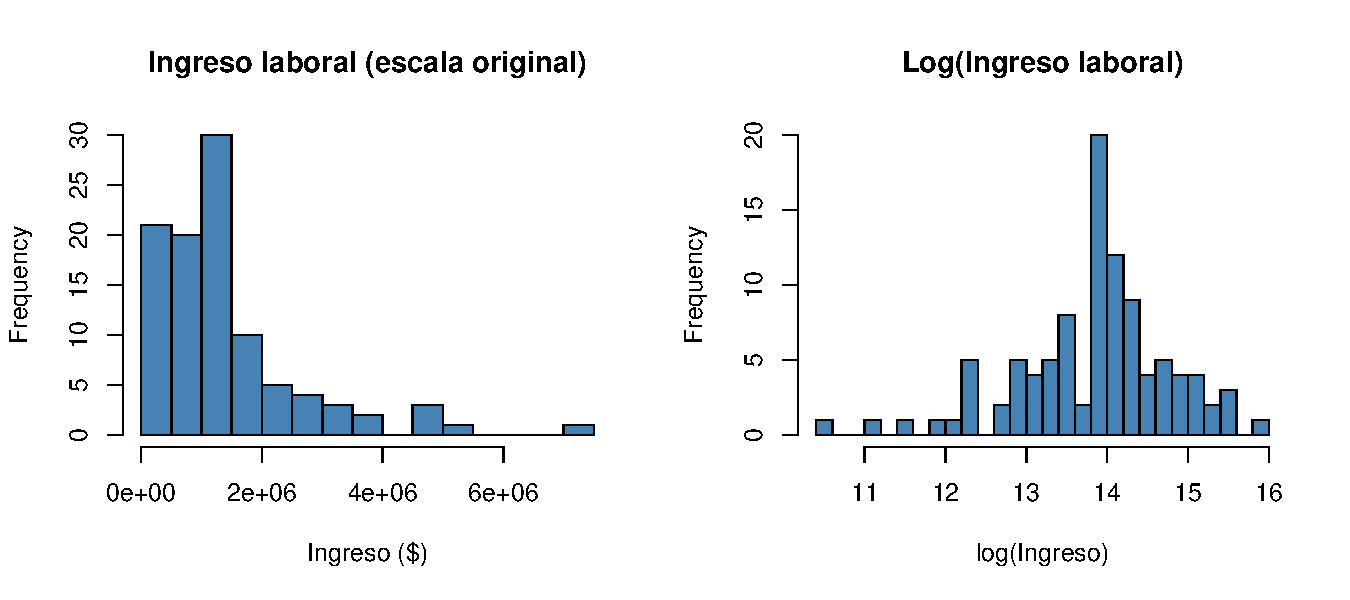
\includegraphics[keepaspectratio]{CatañoCentenoCifuentesRLM_2_files/figure-pdf/hist-y-1.pdf}}

Se muestra el ingreso en su escala original y ya transformado a
logaritmo: el histograma de la izquierda evidencia la asimetría positiva
característica de los ingresos laborales (unos pocos valores muy altos
alargan la cola derecha), mientras que el de la derecha muestra una
distribución considerablemente más simétrica, lo que respalda el uso de
\(\ln(Y)\) como variable de respuesta del modelo.

\subsection{Descripción de las covariables
continuas}\label{descripciuxf3n-de-las-covariables-continuas}

\begin{longtable}[]{@{}lrrrrrrr@{}}
\caption{Estadísticos descriptivos de las covariables continuas (n =
100)}\tabularnewline
\toprule\noalign{}
Variable & Media & Mediana & DE & Min & Max & Q1 & Q3 \\
\midrule\noalign{}
\endfirsthead
\toprule\noalign{}
Variable & Media & Mediana & DE & Min & Max & Q1 & Q3 \\
\midrule\noalign{}
\endhead
\bottomrule\noalign{}
\endlastfoot
antiguedad & 78.19 & 36.0 & 93.26 & 0 & 480 & 12 & 120 \\
edad & 41.38 & 39.0 & 12.81 & 19 & 71 & 32 & 50 \\
edad2 & 1874.86 & 1521.0 & 1144.50 & 361 & 5041 & 1024 & 2500 \\
escolaridad & 11.18 & 11.0 & 4.29 & 0 & 18 & 9 & 14 \\
horas & 42.78 & 47.5 & 13.96 & 3 & 76 & 40 & 48 \\
\end{longtable}

La Tabla 5 muestra asimetrías marcadas entre las covariables continuas.
La antigüedad es la más sesgada: su media (78.19 meses) casi duplica su
mediana (36 meses), y su desviación estándar (93.26) supera a la propia
media, lo que indica una fuerte cola derecha --- la mayoría de los
trabajadores lleva poco tiempo en su empleo actual (Q1 = 12 meses, Q3 =
120 meses), pero un grupo reducido con antigüedades de hasta 480 meses
(40 años) arrastra el promedio hacia arriba. La edad, en cambio,
presenta media y mediana cercanas (41.38 y 39 años) y una dispersión
moderada (DE = 12.81), consistente con una distribución razonablemente
simétrica en el rango de vida laboral activa (19-71 años). La
escolaridad también es prácticamente simétrica (media 11.18, mediana 11
años), con la mitad central de la muestra (Q1-Q3) situada entre 9 y 14
años, es decir, entre bachillerato incompleto y estudios técnicos o
tecnológicos. Las horas trabajadas muestran una mediana (47.5) superior
a la media (42.78), lo que sugiere una cola hacia valores bajos: la
mayoría trabaja entre 40 y 48 horas semanales (Q1-Q3), pero algunos
casos de jornadas muy reducidas (mínimo de 3 horas) bajan el promedio
general.

\begin{figure}

\centering{

\pandocbounded{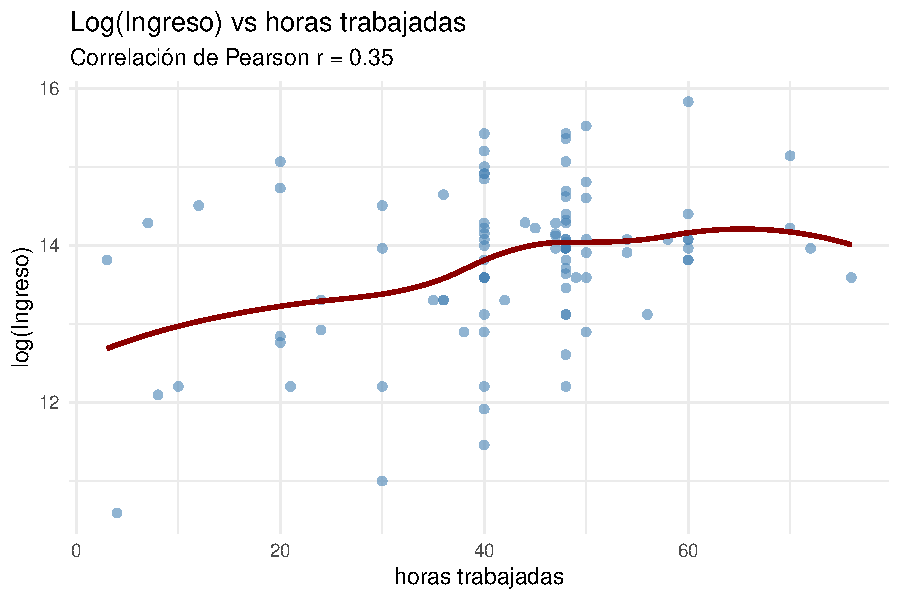
\includegraphics[keepaspectratio]{CatañoCentenoCifuentesRLM_2_files/figure-pdf/fig-scatter-horas-1.pdf}}

}

\caption{\label{fig-scatter-horas}Log(Ingreso) vs.~horas trabajadas por
semana}

\end{figure}%

\begin{figure}

\centering{

\pandocbounded{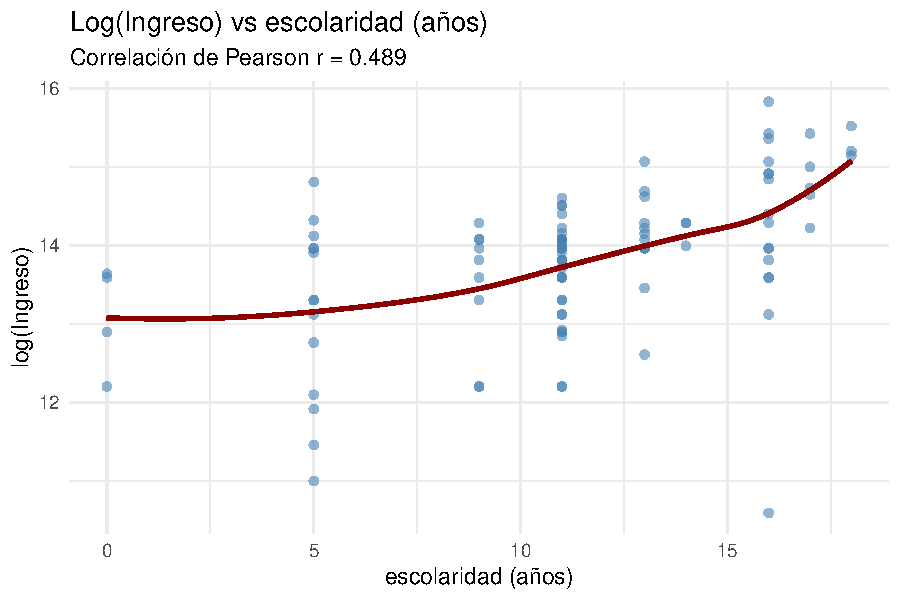
\includegraphics[keepaspectratio]{CatañoCentenoCifuentesRLM_2_files/figure-pdf/fig-scatter-escolaridad-1.pdf}}

}

\caption{\label{fig-scatter-escolaridad}Log(Ingreso) vs.~años de
escolaridad}

\end{figure}%

\begin{figure}

\centering{

\pandocbounded{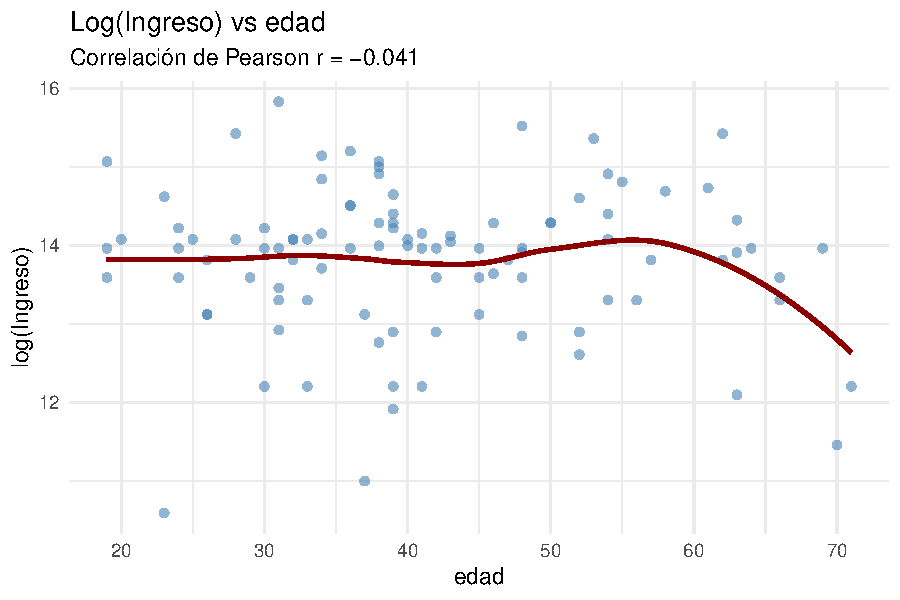
\includegraphics[keepaspectratio]{CatañoCentenoCifuentesRLM_2_files/figure-pdf/fig-scatter-edad-1.pdf}}

}

\caption{\label{fig-scatter-edad}Log(Ingreso) vs.~edad}

\end{figure}%

\begin{figure}

\centering{

\pandocbounded{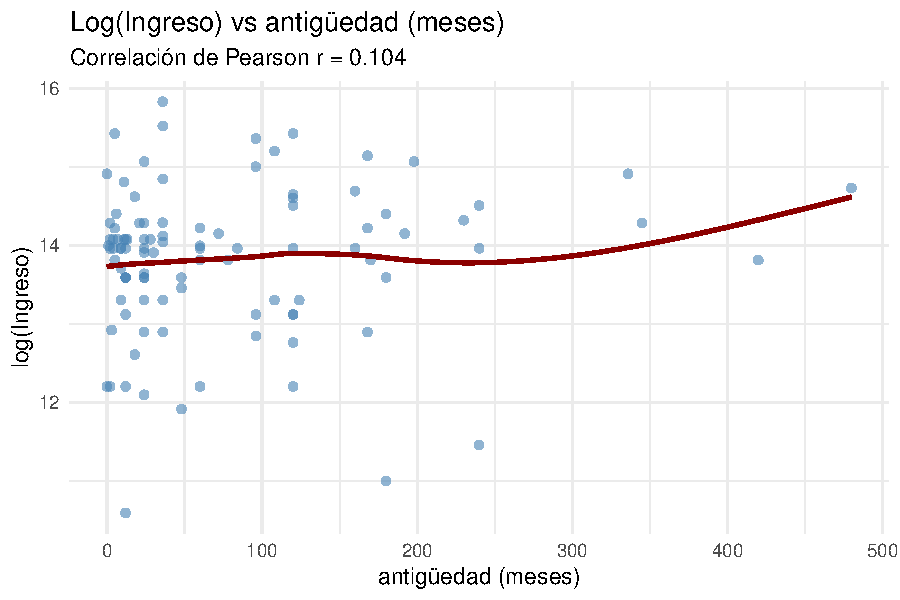
\includegraphics[keepaspectratio]{CatañoCentenoCifuentesRLM_2_files/figure-pdf/fig-scatter-antiguedad-1.pdf}}

}

\caption{\label{fig-scatter-antiguedad}Log(Ingreso) vs.~antigüedad en el
empleo actual}

\end{figure}%

Las Figuras Figura~\ref{fig-scatter-horas} a
Figura~\ref{fig-scatter-antiguedad} muestran la relación entre el
log-ingreso y cada covariable continua, junto con una curva LOESS y el
coeficiente de correlación de Pearson. La escolaridad presenta la
asociación lineal más fuerte con el log-ingreso (r=0.489r = 0.489
r=0.489), con una tendencia creciente y particularmente pronunciada en
los niveles más altos de educación, consistente con los rendimientos
crecientes a la educación superior documentados en la literatura. Las
horas trabajadas muestran una asociación positiva moderada (r=0.350r =
0.350 r=0.350), aunque la curva LOESS evidencia un aplanamiento a partir
de las 40 horas semanales: superado ese umbral, trabajar más horas no se
traduce en incrementos proporcionales del ingreso. La antigüedad exhibe
una correlación lineal débil (r=0.104r = 0.104 r=0.104), con la mayoría
de las observaciones concentradas en valores bajos y un leve repunte
solo en los casos de mayor antigüedad. La edad es el caso más
particular: su correlación de Pearson es prácticamente nula (r=−0.041r =
-0.041 r=−0.041), pero la curva LOESS sí insinúa el perfil cóncavo
esperado por la teoría del capital humano ---un leve ascenso hasta la
quinta década de vida seguido de un descenso---, lo que confirma que la
relación no es de tipo lineal y respalda la inclusión del término
cuadrático (edad²) en el modelo en lugar de depender únicamente del
coeficiente de correlación simple.

Se observa que los puntos de la Figura
Figura~\ref{fig-scatter-escolaridad} se agrupan en un número reducido de
valores discretos (0, 5, 9, 11, 13, 14, 16, 17, 18 y 21 años) en lugar
de distribuirse de forma continua. Esto es consecuencia directa del
método de construcción de la variable: al no preguntarse en la GEIH el
número exacto de años cursados sino el nivel educativo alcanzado, la
escolaridad se aproxima mediante la duración típica asociada a cada
nivel (Ley 115 de 1994 y convención de Núñez \& Sánchez, 1998). Se
trata, por tanto, de una variable discreta con una escala de intervalo
bien definida, tratada como continua siguiendo la convención estándar en
la literatura de determinantes salariales, en la que ``años de
escolaridad'' se modela habitualmente como covariable continua pese a su
naturaleza discreta (Mincer, 1974; Núñez \& Sánchez, 1998).

\begin{longtable}[]{@{}lrrrrr@{}}
\caption{Matriz de correlaciones de Pearson entre las variables
continuas}\tabularnewline
\toprule\noalign{}
& ln\_ingreso & horas & escolaridad & edad & antiguedad \\
\midrule\noalign{}
\endfirsthead
\toprule\noalign{}
& ln\_ingreso & horas & escolaridad & edad & antiguedad \\
\midrule\noalign{}
\endhead
\bottomrule\noalign{}
\endlastfoot
ln\_ingreso & 1.000 & 0.350 & 0.489 & -0.041 & 0.104 \\
horas & 0.350 & 1.000 & -0.012 & -0.093 & -0.313 \\
escolaridad & 0.489 & -0.012 & 1.000 & -0.233 & 0.038 \\
edad & -0.041 & -0.093 & -0.233 & 1.000 & 0.381 \\
antiguedad & 0.104 & -0.313 & 0.038 & 0.381 & 1.000 \\
\end{longtable}

\begin{figure}

\centering{

\pandocbounded{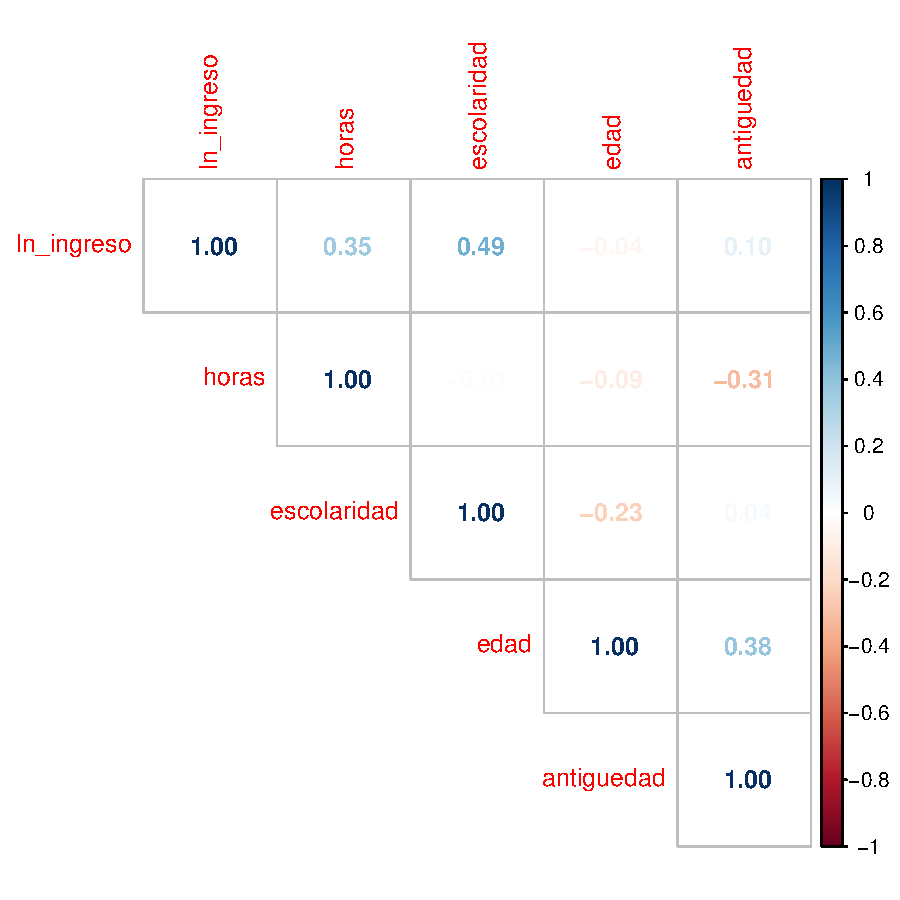
\includegraphics[keepaspectratio]{CatañoCentenoCifuentesRLM_2_files/figure-pdf/fig-corrplot-1.pdf}}

}

\caption{\label{fig-corrplot}Matriz de correlaciones de Pearson entre
las variables continuas (representación gráfica)}

\end{figure}%

La Tabla 6 y la Figura Figura~\ref{fig-corrplot} confirman la jerarquía
observada en los diagramas de dispersión: la escolaridad (0.489) y las
horas trabajadas (0.350) son las covariables más asociadas linealmente
con el log-ingreso, seguidas de la antigüedad (0.104) y la edad
(-0.041). En cuanto a la asociación entre covariables, la mayor
correlación se presenta entre edad y antigüedad (r=0.381r = 0.381
r=0.381), lo cual es esperable dado que ambas están ligadas al ciclo de
vida laboral; también destaca una correlación negativa moderada entre
horas trabajadas y antigüedad (r=−0.313r = -0.313 r=−0.313), y entre
escolaridad y edad (r=−0.233r = -0.233 r=−0.233), esta última
consistente con la expansión histórica del acceso a la educación en
Colombia, que ha elevado la escolaridad promedio de las cohortes más
jóvenes frente a las de mayor edad. Ninguna de estas correlaciones
supera el umbral de 0.5 usualmente considerado como señal de alerta
temprana de multicolinealidad severa, aunque la asociación entre edad y
antigüedad es la que ameritará mayor atención al calcular los VIF en la
etapa de estimación del modelo.

\subsection{Descripción de la variable
categórica}\label{descripciuxf3n-de-la-variable-categuxf3rica}

\subsubsection{Rama de actividad
económica}\label{rama-de-actividad-econuxf3mica}

\begin{longtable}[]{@{}
  >{\raggedright\arraybackslash}p{(\linewidth - 6\tabcolsep) * \real{0.4507}}
  >{\raggedleft\arraybackslash}p{(\linewidth - 6\tabcolsep) * \real{0.0423}}
  >{\raggedleft\arraybackslash}p{(\linewidth - 6\tabcolsep) * \real{0.2394}}
  >{\raggedleft\arraybackslash}p{(\linewidth - 6\tabcolsep) * \real{0.2676}}@{}}
\caption{Distribución de la muestra y log-ingreso medio según sector
económico agregado (n = 100)}\tabularnewline
\toprule\noalign{}
\begin{minipage}[b]{\linewidth}\raggedright
rama
\end{minipage} & \begin{minipage}[b]{\linewidth}\raggedleft
n
\end{minipage} & \begin{minipage}[b]{\linewidth}\raggedleft
Media\_ln\_ingreso
\end{minipage} & \begin{minipage}[b]{\linewidth}\raggedleft
Mediana\_ln\_ingreso
\end{minipage} \\
\midrule\noalign{}
\endfirsthead
\toprule\noalign{}
\begin{minipage}[b]{\linewidth}\raggedright
rama
\end{minipage} & \begin{minipage}[b]{\linewidth}\raggedleft
n
\end{minipage} & \begin{minipage}[b]{\linewidth}\raggedleft
Media\_ln\_ingreso
\end{minipage} & \begin{minipage}[b]{\linewidth}\raggedleft
Mediana\_ln\_ingreso
\end{minipage} \\
\midrule\noalign{}
\endhead
\bottomrule\noalign{}
\endlastfoot
Comercio\_transporte\_alojamiento & 33 & 13.78 & 13.96 \\
Servicios\_sociales\_otros & 24 & 14.19 & 14.11 \\
Industria\_mineria\_construccion & 20 & 13.94 & 14.02 \\
Agropecuario & 12 & 13.21 & 13.21 \\
Servicios\_financ\_profesionales & 11 & 13.61 & 13.96 \\
\end{longtable}

La recodificación en cinco sectores agregados produjo una distribución
mucho más manejable que la original: el grupo más grande, Comercio,
transporte y alojamiento, concentra 33 observaciones, seguido de
Servicios sociales y otros (24) e Industria, minería y construcción
(20). Agropecuario reúne 12 observaciones y Servicios financieros y
profesionales, el grupo más pequeño, queda con 11 --- sensiblemente
mejor que los 18 grupos con una sola observación que tenía la
codificación original, aunque este último grupo sigue siendo el más
vulnerable a la inestabilidad muestral y deberá vigilarse en la etapa de
estimación (por ejemplo, revisando su apalancamiento e influencia sobre
el modelo). En cuanto al log-ingreso medio, Servicios sociales y otros
presenta el valor más alto (media 14.19, mediana 14.11), seguido de
cerca por Industria, minería y construcción (13.94 y 14.02); en el otro
extremo, Agropecuario registra el log-ingreso medio más bajo (13.21,
mediana 13.21). Comercio, transporte y alojamiento ---pese a ser el
sector con más observaciones--- y Servicios financieros y profesionales
quedan en un nivel intermedio, con medias de 13.78 y 13.61
respectivamente, y medianas prácticamente iguales (13.96 en ambos
casos).

\begin{figure}

\centering{

\pandocbounded{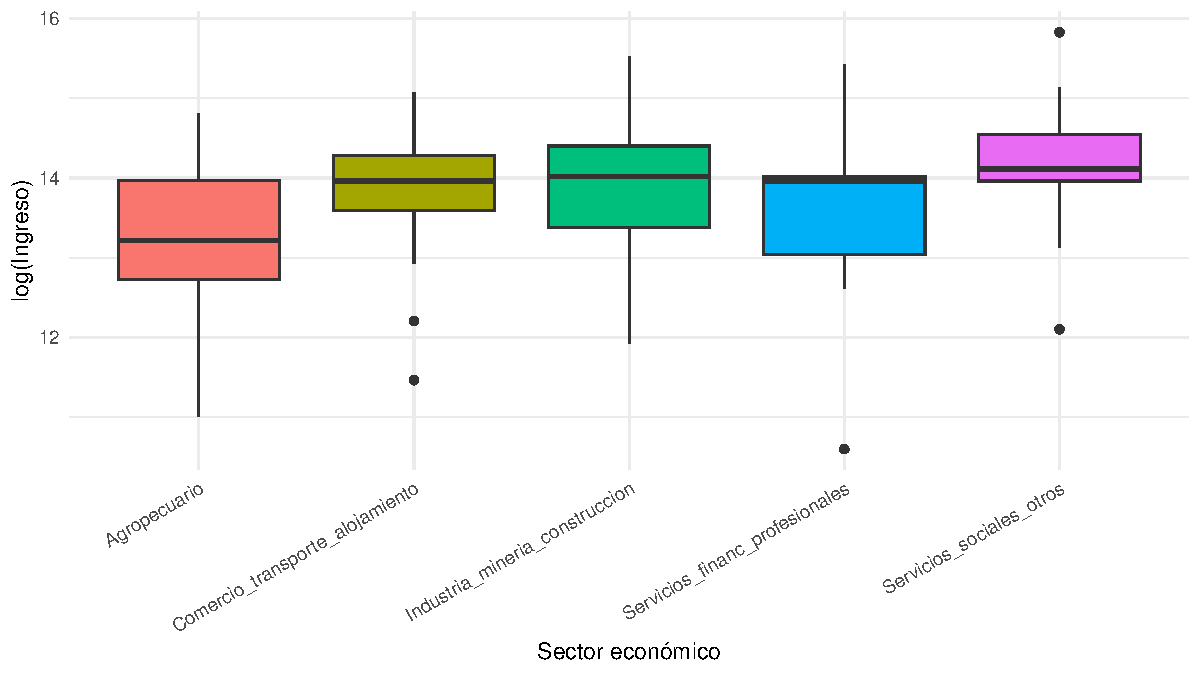
\includegraphics[keepaspectratio]{CatañoCentenoCifuentesRLM_2_files/figure-pdf/fig-rama-1.pdf}}

}

\caption{\label{fig-rama}Log(Ingreso) según sector económico agregado}

\end{figure}%

La Figura 6 confirma la heterogeneidad sectorial sugerida por la Tabla 7
(nótese que el eje horizontal ordena los sectores alfabéticamente y no
por tamaño muestral). Servicios sociales y otros presenta la mediana más
alta y la caja más compacta de los cinco sectores ---es decir, la menor
dispersión en el 50\% central de sus datos---, aunque exhibe dos valores
atípicos: uno muy alto, el mayor de toda la muestra, y otro bajo, que
amplían su rango total pese a la estrechez de la caja. Industria,
minería y construcción tiene la segunda mediana más alta y, a diferencia
del sector anterior, no presenta valores atípicos, si bien sus bigotes
cubren un rango amplio. Comercio, transporte y alojamiento y Servicios
financieros y profesionales muestran medianas muy similares entre sí y
ligeramente por debajo de Industria, consistentes con el empate
observado en la Tabla 7 (13.96 en ambos casos); el primero registra dos
valores atípicos bajos y el segundo uno solo, más extremo, que
corresponde al valor mínimo de toda la muestra. Agropecuario registra la
mediana más baja de los cinco sectores y la caja de mayor altura, lo que
indica una mayor heterogeneidad interna en su 50\% central, sin valores
atípicos marcados. En conjunto, la brecha entre el sector con mayor
log-ingreso medio (Servicios sociales y otros, 14.19) y el de menor
log-ingreso medio (Agropecuario, 13.21) es de 0.98 puntos en escala
logarítmica, una diferencia sustancial que respalda la Hipótesis 2 sobre
la existencia de brechas de ingreso asociadas al sector económico,
aunque su significancia estadística formal deberá confirmarse en la
etapa de estimación del modelo, controlando por escolaridad, edad, horas
trabajadas y antigüedad.

\section{Estimación del modelo con covariables
continuas}\label{estimaciuxf3n-del-modelo-con-covariables-continuas}

\subsection{Ajuste del modelo}\label{ajuste-del-modelo}

\begin{Shaded}
\begin{Highlighting}[]
\NormalTok{modelo\_continuas }\OtherTok{\textless{}{-}} \FunctionTok{lm}\NormalTok{(ln\_ingreso }\SpecialCharTok{\textasciitilde{}}\NormalTok{ horas }\SpecialCharTok{+}\NormalTok{ escolaridad }\SpecialCharTok{+}\NormalTok{ edad }\SpecialCharTok{+}\NormalTok{ edad2 }\SpecialCharTok{+}\NormalTok{ antiguedad,}
                        \AttributeTok{data =}\NormalTok{ muestra)}
\FunctionTok{summary}\NormalTok{(modelo\_continuas)}
\end{Highlighting}
\end{Shaded}

\begin{verbatim}

Call:
lm(formula = ln_ingreso ~ horas + escolaridad + edad + edad2 + 
    antiguedad, data = muestra)

Residuals:
     Min       1Q   Median       3Q      Max 
-2.43540 -0.36965  0.03507  0.45412  1.90504 

Coefficients:
              Estimate Std. Error t value Pr(>|t|)    
(Intercept)  1.097e+01  8.028e-01  13.659  < 2e-16 ***
horas        2.871e-02  5.728e-03   5.012 2.52e-06 ***
escolaridad  1.093e-01  1.834e-02   5.957 4.42e-08 ***
edad         9.561e-03  3.676e-02   0.260   0.7953    
edad2       -7.814e-05  4.112e-04  -0.190   0.8497    
antiguedad   2.064e-03  9.260e-04   2.228   0.0282 *  
---
Signif. codes:  0 '***' 0.001 '**' 0.01 '*' 0.05 '.' 0.1 ' ' 1

Residual standard error: 0.7487 on 94 degrees of freedom
Multiple R-squared:  0.4106,    Adjusted R-squared:  0.3793 
F-statistic:  13.1 on 5 and 94 DF,  p-value: 1.122e-09
\end{verbatim}

\begin{longtable}[]{@{}lrrrr@{}}
\caption{Parámetros estimados del modelo con covariables
continuas}\tabularnewline
\toprule\noalign{}
Parámetro & Estimación & Error estándar & t & p-valor \\
\midrule\noalign{}
\endfirsthead
\toprule\noalign{}
Parámetro & Estimación & Error estándar & t & p-valor \\
\midrule\noalign{}
\endhead
\bottomrule\noalign{}
\endlastfoot
(Intercept) & 10.9656 & 0.8028 & 13.659 & 0.0000 \\
horas & 0.0287 & 0.0057 & 5.012 & 0.0000 \\
escolaridad & 0.1093 & 0.0183 & 5.957 & 0.0000 \\
edad & 0.0096 & 0.0368 & 0.260 & 0.7953 \\
edad2 & -0.0001 & 0.0004 & -0.190 & 0.8497 \\
antiguedad & 0.0021 & 0.0009 & 2.228 & 0.0282 \\
\end{longtable}

La ecuación ajustada es:

\[
\widehat{\ln(Y_i)} = 10.97 + 0.0287\,X_{1i} + 0.1093\,X_{2i} + 0.0096\,X_{3i} - 0.000078\,X_{4i} + 0.00206\,X_{5i}
\]

donde \(X_1\): horas, \(X_2\): escolaridad, \(X_3\): edad, \(X_4\):
edad², \(X_5\): antigüedad.

\subsection{ANOVA del modelo}\label{anova-del-modelo}

\begin{longtable}[]{@{}lrrrrr@{}}
\caption{Tabla ANOVA del modelo con covariables
continuas}\tabularnewline
\toprule\noalign{}
Fuente & Df & Sum Sq & Mean Sq & F value & Pr(\textgreater F) \\
\midrule\noalign{}
\endfirsthead
\toprule\noalign{}
Fuente & Df & Sum Sq & Mean Sq & F value & Pr(\textgreater F) \\
\midrule\noalign{}
\endhead
\bottomrule\noalign{}
\endlastfoot
horas & 1 & 10.9825 & 10.9825 & 19.5908 & 0.0000 \\
escolaridad & 1 & 21.7831 & 21.7831 & 38.8570 & 0.0000 \\
edad & 1 & 1.0994 & 1.0994 & 1.9611 & 0.1647 \\
edad2 & 1 & 0.0627 & 0.0627 & 0.1118 & 0.7388 \\
antiguedad & 1 & 2.7839 & 2.7839 & 4.9660 & 0.0282 \\
Residuals & 94 & 52.6961 & 0.5606 & NA & NA \\
\end{longtable}

El estadístico F global es de 13.097 con 5 y 94 grados de libertad, con
un p-valor de 1.12e-09. El modelo explica el 41.06\% de la variabilidad
total del log-ingreso (\(R^2=\) 0.4106; \(R^2\) ajustado \(=\) 0.3793).

\subsection{Interpretación rigurosa}\label{interpretaciuxf3n-rigurosa}

¿Es significativo el modelo? Sí, de forma inequívoca. La hipótesis nula
del ANOVA global (todos los \(\beta=0\) excepto el intercepto) se
rechaza con un p-valor prácticamente nulo. Al menos una covariable tiene
poder explicativo real sobre el log-ingreso.

Pero ``significativo globalmente'' no es lo mismo que ``todas las
variables aportan''. Mirando los coeficientes individuales: horas,
escolaridad y antigüedad son significativas al 5\% (antigüedad justo en
el límite, \(p=0.028\)); edad y edad² no lo son en absoluto (\(p=0.795\)
y \(p=0.850\)). Esto es coherente con lo que ya se había anticipado en
el análisis descriptivo: la correlación de Pearson entre edad y
log-ingreso era prácticamente nula (\(r=-0.041\)), y aunque la curva
LOESS insinuaba un perfil cóncavo, aquí ---controlando por las demás
variables--- ese efecto no resulta estadísticamente detectable con
\(n=100\). Esto es un llamado de atención sobre la Hipótesis 1: la
escolaridad sí se confirma (\(\beta_2>0\), \(p<0.001\)), pero el
componente de edad de la hipótesis no se sostiene en este modelo
reducido.

Sobre el 41.06\% de varianza explicada, es importante no
sobre-interpretar ni subestimar:

\begin{itemize}
\tightlist
\item
  Para datos de corte transversal en economía laboral con encuestas de
  hogares, un \(R^2\) de \textasciitilde0.41 no es bajo --- es habitual
  que ecuaciones de Mincer con variables individuales expliquen entre
  20\% y 40\% de la varianza del log-salario, porque el ingreso
  individual depende de muchísimos factores no observados (habilidad,
  calidad del empleador, negociación, informalidad, etc.) que ninguna
  encuesta captura.
\item
  Sin embargo, queda un 59\% sin explicar, y el propio análisis
  descriptivo del documento (Tabla 7, Figura 6) ya había detectado que
  la rama de actividad económica genera diferencias sustanciales (brecha
  de 0.98 puntos log entre sectores) que este modelo reducido no
  incorpora. Es razonable esperar que al añadir la variable categórica
  rama (el modelo completo con \(X_6\)) el \(R^2\) aumente y que parte
  de la varianza residual se explique por heterogeneidad sectorial.
\item
  Con \(n=100\), el \(R^2\) ajustado (0.379) es la medida más honesta
  porque penaliza los 5 grados de libertad consumidos; la caída de 0.41
  a 0.38 no es dramática, así que el modelo no está sobreajustado por el
  número de covariables.
\item
  Dado que edad y edad² no aportan significancia, valdría la pena ---en
  la etapa de selección de modelo--- evaluar si conviene mantenerlas por
  justificación teórica (Mincer) pese a su no significancia, o si su
  falta de poder explicativo aquí se debe a la correlación moderada con
  antigüedad (\(r=0.381\)) generando cierta redundancia entre esas dos
  variables.
\end{itemize}

\section{Selección de modelos (covariables
continuas)}\label{selecciuxf3n-de-modelos-covariables-continuas}

\begin{Shaded}
\begin{Highlighting}[]
\FunctionTok{library}\NormalTok{(leaps)}
\end{Highlighting}
\end{Shaded}

\begin{verbatim}
Warning: package 'leaps' was built under R version 4.6.1
\end{verbatim}

\begin{Shaded}
\begin{Highlighting}[]
\NormalTok{modelo\_nulo }\OtherTok{\textless{}{-}} \FunctionTok{lm}\NormalTok{(ln\_ingreso }\SpecialCharTok{\textasciitilde{}} \DecValTok{1}\NormalTok{, }\AttributeTok{data =}\NormalTok{ muestra)}
\CommentTok{\# modelo\_continuas ya fue definido antes:}
\CommentTok{\# modelo\_continuas \textless{}{-} lm(ln\_ingreso \textasciitilde{} horas + escolaridad + edad + edad2 + antiguedad, data = muestra)}
\end{Highlighting}
\end{Shaded}

\subsection{\texorpdfstring{a) Selección por
\(R^2_{adj}\)}{a) Selección por R\^{}2\_\{adj\}}}\label{a-selecciuxf3n-por-r2_adj}

\begin{Shaded}
\begin{Highlighting}[]
\NormalTok{best }\OtherTok{\textless{}{-}} \FunctionTok{regsubsets}\NormalTok{(ln\_ingreso }\SpecialCharTok{\textasciitilde{}}\NormalTok{ horas }\SpecialCharTok{+}\NormalTok{ escolaridad }\SpecialCharTok{+}\NormalTok{ edad }\SpecialCharTok{+}\NormalTok{ edad2 }\SpecialCharTok{+}\NormalTok{ antiguedad,}
                    \AttributeTok{data =}\NormalTok{ muestra, }\AttributeTok{nvmax =} \DecValTok{5}\NormalTok{)}
\NormalTok{sm }\OtherTok{\textless{}{-}} \FunctionTok{summary}\NormalTok{(best)}

\FunctionTok{kable}\NormalTok{(}\FunctionTok{data.frame}\NormalTok{(}\AttributeTok{Num\_predictores =} \DecValTok{1}\SpecialCharTok{:}\DecValTok{5}\NormalTok{, }\AttributeTok{R2\_ajustado =} \FunctionTok{round}\NormalTok{(sm}\SpecialCharTok{$}\NormalTok{adjr2, }\DecValTok{4}\NormalTok{)),}
      \AttributeTok{caption =} \StringTok{"Resumen de selección por R2 ajustado"}\NormalTok{)}
\end{Highlighting}
\end{Shaded}

\begin{longtable}[]{@{}rr@{}}
\caption{Resumen de selección por R2 ajustado}\tabularnewline
\toprule\noalign{}
Num\_predictores & R2\_ajustado \\
\midrule\noalign{}
\endfirsthead
\toprule\noalign{}
Num\_predictores & R2\_ajustado \\
\midrule\noalign{}
\endhead
\bottomrule\noalign{}
\endlastfoot
1 & 0.2316 \\
2 & 0.3534 \\
3 & 0.3909 \\
4 & 0.3856 \\
5 & 0.3793 \\
\end{longtable}

\begin{Shaded}
\begin{Highlighting}[]
\NormalTok{modelo\_r2adj }\OtherTok{\textless{}{-}} \FunctionTok{lm}\NormalTok{(ln\_ingreso }\SpecialCharTok{\textasciitilde{}}\NormalTok{ horas }\SpecialCharTok{+}\NormalTok{ escolaridad }\SpecialCharTok{+}\NormalTok{ antiguedad, }\AttributeTok{data =}\NormalTok{ muestra)}
\end{Highlighting}
\end{Shaded}

\begin{longtable}[]{@{}lrrrrr@{}}
\caption{ANOVA - modelo por R2 ajustado}\tabularnewline
\toprule\noalign{}
& Df & Sum Sq & Mean Sq & F value & Pr(\textgreater F) \\
\midrule\noalign{}
\endfirsthead
\toprule\noalign{}
& Df & Sum Sq & Mean Sq & F value & Pr(\textgreater F) \\
\midrule\noalign{}
\endhead
\bottomrule\noalign{}
\endlastfoot
horas & 1 & 10.9825 & 10.9825 & 19.9646 & 0.0000 \\
escolaridad & 1 & 21.7831 & 21.7831 & 39.5985 & 0.0000 \\
antiguedad & 1 & 3.8326 & 3.8326 & 6.9670 & 0.0097 \\
Residuals & 96 & 52.8096 & 0.5501 & NA & NA \\
\end{longtable}

\begin{longtable}[]{@{}lrrrr@{}}
\caption{Parámetros - modelo por R2 ajustado}\tabularnewline
\toprule\noalign{}
& Estimate & Std. Error & t value &
Pr(\textgreater\textbar t\textbar) \\
\midrule\noalign{}
\endfirsthead
\toprule\noalign{}
& Estimate & Std. Error & t value &
Pr(\textgreater\textbar t\textbar) \\
\midrule\noalign{}
\endhead
\bottomrule\noalign{}
\endlastfoot
(Intercept) & 11.2109 & 0.3384 & 33.1275 & 0.0000 \\
horas & 0.0289 & 0.0056 & 5.1428 & 0.0000 \\
escolaridad & 0.1077 & 0.0174 & 6.1941 & 0.0000 \\
antiguedad & 0.0022 & 0.0008 & 2.6395 & 0.0097 \\
\end{longtable}

\subsection{\texorpdfstring{b) Selección por \(C_p\) de
Mallows}{b) Selección por C\_p de Mallows}}\label{b-selecciuxf3n-por-c_p-de-mallows}

\begin{Shaded}
\begin{Highlighting}[]
\FunctionTok{kable}\NormalTok{(}\FunctionTok{data.frame}\NormalTok{(}\AttributeTok{Num\_predictores =} \DecValTok{1}\SpecialCharTok{:}\DecValTok{5}\NormalTok{, }\AttributeTok{Cp =} \FunctionTok{round}\NormalTok{(sm}\SpecialCharTok{$}\NormalTok{cp, }\DecValTok{4}\NormalTok{)),}
      \AttributeTok{caption =} \StringTok{"Resumen de selección por Cp de Mallows"}\NormalTok{)}
\end{Highlighting}
\end{Shaded}

\begin{longtable}[]{@{}rr@{}}
\caption{Resumen de selección por Cp de Mallows}\tabularnewline
\toprule\noalign{}
Num\_predictores & Cp \\
\midrule\noalign{}
\endfirsthead
\toprule\noalign{}
Num\_predictores & Cp \\
\midrule\noalign{}
\endhead
\bottomrule\noalign{}
\endlastfoot
1 & 25.3124 \\
2 & 7.0389 \\
3 & 2.2023 \\
4 & 4.0361 \\
5 & 6.0000 \\
\end{longtable}

\begin{Shaded}
\begin{Highlighting}[]
\NormalTok{modelo\_cp }\OtherTok{\textless{}{-}} \FunctionTok{lm}\NormalTok{(ln\_ingreso }\SpecialCharTok{\textasciitilde{}}\NormalTok{ horas }\SpecialCharTok{+}\NormalTok{ escolaridad }\SpecialCharTok{+}\NormalTok{ antiguedad, }\AttributeTok{data =}\NormalTok{ muestra)}
\end{Highlighting}
\end{Shaded}

\begin{longtable}[]{@{}lrrrrr@{}}
\caption{ANOVA - modelo por Cp}\tabularnewline
\toprule\noalign{}
& Df & Sum Sq & Mean Sq & F value & Pr(\textgreater F) \\
\midrule\noalign{}
\endfirsthead
\toprule\noalign{}
& Df & Sum Sq & Mean Sq & F value & Pr(\textgreater F) \\
\midrule\noalign{}
\endhead
\bottomrule\noalign{}
\endlastfoot
horas & 1 & 10.9825 & 10.9825 & 19.9646 & 0.0000 \\
escolaridad & 1 & 21.7831 & 21.7831 & 39.5985 & 0.0000 \\
antiguedad & 1 & 3.8326 & 3.8326 & 6.9670 & 0.0097 \\
Residuals & 96 & 52.8096 & 0.5501 & NA & NA \\
\end{longtable}

\begin{longtable}[]{@{}lrrrr@{}}
\caption{Parámetros - modelo por Cp}\tabularnewline
\toprule\noalign{}
& Estimate & Std. Error & t value &
Pr(\textgreater\textbar t\textbar) \\
\midrule\noalign{}
\endfirsthead
\toprule\noalign{}
& Estimate & Std. Error & t value &
Pr(\textgreater\textbar t\textbar) \\
\midrule\noalign{}
\endhead
\bottomrule\noalign{}
\endlastfoot
(Intercept) & 11.2109 & 0.3384 & 33.1275 & 0.0000 \\
horas & 0.0289 & 0.0056 & 5.1428 & 0.0000 \\
escolaridad & 0.1077 & 0.0174 & 6.1941 & 0.0000 \\
antiguedad & 0.0022 & 0.0008 & 2.6395 & 0.0097 \\
\end{longtable}

\subsection{c) Stepwise (ambas direcciones,
AIC)}\label{c-stepwise-ambas-direcciones-aic}

\begin{Shaded}
\begin{Highlighting}[]
\NormalTok{modelo\_stepwise }\OtherTok{\textless{}{-}} \FunctionTok{step}\NormalTok{(modelo\_continuas, }\AttributeTok{direction =} \StringTok{"both"}\NormalTok{, }\AttributeTok{trace =} \DecValTok{0}\NormalTok{)}
\FunctionTok{formula}\NormalTok{(modelo\_stepwise)}
\end{Highlighting}
\end{Shaded}

\begin{verbatim}
ln_ingreso ~ horas + escolaridad + antiguedad
\end{verbatim}

\begin{longtable}[]{@{}lrrrrr@{}}
\caption{ANOVA - modelo Stepwise}\tabularnewline
\toprule\noalign{}
& Df & Sum Sq & Mean Sq & F value & Pr(\textgreater F) \\
\midrule\noalign{}
\endfirsthead
\toprule\noalign{}
& Df & Sum Sq & Mean Sq & F value & Pr(\textgreater F) \\
\midrule\noalign{}
\endhead
\bottomrule\noalign{}
\endlastfoot
horas & 1 & 10.9825 & 10.9825 & 19.9646 & 0.0000 \\
escolaridad & 1 & 21.7831 & 21.7831 & 39.5985 & 0.0000 \\
antiguedad & 1 & 3.8326 & 3.8326 & 6.9670 & 0.0097 \\
Residuals & 96 & 52.8096 & 0.5501 & NA & NA \\
\end{longtable}

\begin{longtable}[]{@{}lrrrr@{}}
\caption{Parámetros - modelo Stepwise}\tabularnewline
\toprule\noalign{}
& Estimate & Std. Error & t value &
Pr(\textgreater\textbar t\textbar) \\
\midrule\noalign{}
\endfirsthead
\toprule\noalign{}
& Estimate & Std. Error & t value &
Pr(\textgreater\textbar t\textbar) \\
\midrule\noalign{}
\endhead
\bottomrule\noalign{}
\endlastfoot
(Intercept) & 11.2109 & 0.3384 & 33.1275 & 0.0000 \\
horas & 0.0289 & 0.0056 & 5.1428 & 0.0000 \\
escolaridad & 0.1077 & 0.0174 & 6.1941 & 0.0000 \\
antiguedad & 0.0022 & 0.0008 & 2.6395 & 0.0097 \\
\end{longtable}

\subsection{d) Selección hacia adelante
(Forward)}\label{d-selecciuxf3n-hacia-adelante-forward}

\begin{Shaded}
\begin{Highlighting}[]
\NormalTok{modelo\_forward }\OtherTok{\textless{}{-}} \FunctionTok{step}\NormalTok{(modelo\_nulo,}
                        \AttributeTok{scope =} \FunctionTok{list}\NormalTok{(}\AttributeTok{lower =}\NormalTok{ modelo\_nulo, }\AttributeTok{upper =}\NormalTok{ modelo\_continuas),}
                        \AttributeTok{direction =} \StringTok{"forward"}\NormalTok{, }\AttributeTok{trace =} \DecValTok{0}\NormalTok{)}
\FunctionTok{formula}\NormalTok{(modelo\_forward)}
\end{Highlighting}
\end{Shaded}

\begin{verbatim}
ln_ingreso ~ escolaridad + horas + antiguedad
\end{verbatim}

\begin{longtable}[]{@{}lrrrrr@{}}
\caption{ANOVA - modelo Forward}\tabularnewline
\toprule\noalign{}
& Df & Sum Sq & Mean Sq & F value & Pr(\textgreater F) \\
\midrule\noalign{}
\endfirsthead
\toprule\noalign{}
& Df & Sum Sq & Mean Sq & F value & Pr(\textgreater F) \\
\midrule\noalign{}
\endhead
\bottomrule\noalign{}
\endlastfoot
escolaridad & 1 & 21.4004 & 21.4004 & 38.9027 & 0.0000 \\
horas & 1 & 11.3653 & 11.3653 & 20.6604 & 0.0000 \\
antiguedad & 1 & 3.8326 & 3.8326 & 6.9670 & 0.0097 \\
Residuals & 96 & 52.8096 & 0.5501 & NA & NA \\
\end{longtable}

\begin{longtable}[]{@{}lrrrr@{}}
\caption{Parámetros - modelo Forward}\tabularnewline
\toprule\noalign{}
& Estimate & Std. Error & t value &
Pr(\textgreater\textbar t\textbar) \\
\midrule\noalign{}
\endfirsthead
\toprule\noalign{}
& Estimate & Std. Error & t value &
Pr(\textgreater\textbar t\textbar) \\
\midrule\noalign{}
\endhead
\bottomrule\noalign{}
\endlastfoot
(Intercept) & 11.2109 & 0.3384 & 33.1275 & 0.0000 \\
escolaridad & 0.1077 & 0.0174 & 6.1941 & 0.0000 \\
horas & 0.0289 & 0.0056 & 5.1428 & 0.0000 \\
antiguedad & 0.0022 & 0.0008 & 2.6395 & 0.0097 \\
\end{longtable}

\subsection{e) Selección hacia atrás
(Backward)}\label{e-selecciuxf3n-hacia-atruxe1s-backward}

\begin{Shaded}
\begin{Highlighting}[]
\NormalTok{modelo\_backward }\OtherTok{\textless{}{-}} \FunctionTok{step}\NormalTok{(modelo\_continuas, }\AttributeTok{direction =} \StringTok{"backward"}\NormalTok{, }\AttributeTok{trace =} \DecValTok{0}\NormalTok{)}
\FunctionTok{formula}\NormalTok{(modelo\_backward)}
\end{Highlighting}
\end{Shaded}

\begin{verbatim}
ln_ingreso ~ horas + escolaridad + antiguedad
\end{verbatim}

\begin{longtable}[]{@{}lrrrrr@{}}
\caption{ANOVA - modelo Backward}\tabularnewline
\toprule\noalign{}
& Df & Sum Sq & Mean Sq & F value & Pr(\textgreater F) \\
\midrule\noalign{}
\endfirsthead
\toprule\noalign{}
& Df & Sum Sq & Mean Sq & F value & Pr(\textgreater F) \\
\midrule\noalign{}
\endhead
\bottomrule\noalign{}
\endlastfoot
horas & 1 & 10.9825 & 10.9825 & 19.9646 & 0.0000 \\
escolaridad & 1 & 21.7831 & 21.7831 & 39.5985 & 0.0000 \\
antiguedad & 1 & 3.8326 & 3.8326 & 6.9670 & 0.0097 \\
Residuals & 96 & 52.8096 & 0.5501 & NA & NA \\
\end{longtable}

\begin{longtable}[]{@{}lrrrr@{}}
\caption{Parámetros - modelo Backward}\tabularnewline
\toprule\noalign{}
& Estimate & Std. Error & t value &
Pr(\textgreater\textbar t\textbar) \\
\midrule\noalign{}
\endfirsthead
\toprule\noalign{}
& Estimate & Std. Error & t value &
Pr(\textgreater\textbar t\textbar) \\
\midrule\noalign{}
\endhead
\bottomrule\noalign{}
\endlastfoot
(Intercept) & 11.2109 & 0.3384 & 33.1275 & 0.0000 \\
horas & 0.0289 & 0.0056 & 5.1428 & 0.0000 \\
escolaridad & 0.1077 & 0.0174 & 6.1941 & 0.0000 \\
antiguedad & 0.0022 & 0.0008 & 2.6395 & 0.0097 \\
\end{longtable}

\subsection{Conclusión sobre la selección de
modelos}\label{conclusiuxf3n-sobre-la-selecciuxf3n-de-modelos}

La aplicación conjunta de los cinco métodos de selección
---\(R^2_{adj}\), \(C_p\) de Mallows, \emph{stepwise}, selección hacia
adelante y selección hacia atrás--- sobre el conjunto de covariables
continuas produjo un resultado inusualmente concluyente: los cinco
métodos convergen exactamente en el mismo modelo final, compuesto por
horas trabajadas, escolaridad y antigüedad en el empleo actual, con
exclusión sistemática de la edad y su término cuadrático. El criterio de
\(R^2_{adj}\) alcanzó su máximo (0.3909) precisamente en el modelo de
tres predictores, tras incrementarse desde 0.2316 (un predictor) y
0.3534 (dos predictores), y decrecer nuevamente al incorporar edad
(0.3856) o edad y edad² (0.3793); de forma análoga, el estadístico
\(C_p\) tocó su mínimo (2.20) en ese mismo modelo de tres variables
---valor cercano a \(p=4\), lo que indica un sesgo estimado
prácticamente nulo respecto al modelo saturado---, frente a valores de
25.31, 7.04, 4.04 y 6.00 para los modelos de una, dos, cuatro y cinco
variables, respectivamente. Las búsquedas secuenciales por AIC
(\emph{stepwise}, \emph{forward} y \emph{backward}) reprodujeron la
misma trayectoria y el mismo punto de convergencia, retirando primero
edad² y luego edad en cada una de sus iteraciones.

El modelo resultante,

\[\widehat{\ln(Y_i)} = 11.21 + 0.0289\,\text{horas}_i + 0.1077\,\text{escolaridad}_i + 0.00222\,\text{antigüedad}_i,\]

es globalmente significativo (\(F_{(3,96)}=22.18\), \(p<0.001\)) y
explica el 40.93 \% de la variabilidad del log-ingreso
(\(R^2_{adj}=0.3909\)), una pérdida marginal de apenas 1.13 puntos
porcentuales de \(R^2\) respecto al modelo completo de cinco covariables
(41.06 \%), lo que confirma que edad y edad² aportaban una fracción de
varianza prácticamente despreciable. Los tres coeficientes retenidos son
individualmente significativos al 5 \% ---horas (\(\hat\beta=0.0289\),
\(p<0.001\)), escolaridad (\(\hat\beta=0.1077\), \(p<0.001\)) y
antigüedad (\(\hat\beta=0.00222\), \(p=0.0097\))---, de modo que ninguna
variable sobrevive en el modelo por mero artificio del procedimiento de
búsqueda.

Este resultado obliga a matizar la Hipótesis 1 planteada en la Sección
6.1. La componente de escolaridad se confirma con solidez: su
coeficiente conserva el signo positivo esperado por la teoría del
capital humano y es el más significativo de los tres retenidos. Sin
embargo, la componente de edad ---tanto en su efecto lineal como en el
cuadrático que debía capturar el perfil cóncavo de la ecuación de
Mincer--- no se sostiene: ya en el modelo completo sus coeficientes no
eran significativos (\(p=0.795\) para edad y \(p=0.850\) para edad²,
Sección ``Estimación del modelo''), y los cinco métodos de selección
coinciden en descartarla por completo. Esto no implica necesariamente
que la relación edad-ingreso sea inexistente en la población de
trabajadores colombianos ---la curva LOESS de la Figura 3 sí insinuaba
visualmente el ascenso y posterior descenso esperado---, sino que, con
una muestra de apenas \(n=100\) observaciones y una correlación de
Pearson entre edad y log-ingreso prácticamente nula (\(r=-0.041\)), el
efecto no resulta estadísticamente detectable una vez controlado por
escolaridad, horas trabajadas y antigüedad. La unanimidad de los cinco
criterios de selección ---que difieren en su lógica (ajuste penalizado,
sesgo respecto al modelo completo, y búsqueda secuencial por
verosimilitud) pero llegan al mismo resultado--- constituye evidencia
razonablemente robusta de que el modelo reducido de tres variables es,
con los datos disponibles, la especificación más parsimoniosa y
defendible, sin que ello descarte que una muestra de mayor tamaño
pudiera revelar el efecto no lineal de la edad que la teoría anticipa.

\section{Conclusiones}\label{conclusiones}

El análisis descriptivo confirma que la transformación logarítmica del
ingreso laboral corrige de forma considerable la asimetría propia de
esta variable (asimetría de -0.785 en el log-ingreso, frente a la
marcada cola derecha visible en la escala original), lo que respalda su
uso como variable de respuesta del modelo.

Entre las covariables continuas, la escolaridad es la que muestra la
asociación lineal más fuerte con el log-ingreso (\(r = 0.489\)), seguida
por las horas trabajadas (\(r = 0.350\)), aunque esta última se aplana a
partir de las 40 horas semanales, indicando rendimientos decrecientes de
la intensidad laboral sobre el ingreso. La antigüedad presenta una
correlación lineal débil (\(r = 0.104\)) y una distribución fuertemente
asimétrica (media de 78.19 meses frente a una mediana de 36), mientras
que la edad exhibe una correlación de Pearson prácticamente nula
(\(r = -0.041\)), pese a que la curva LOESS insinúa el perfil cóncavo
esperado por la teoría del capital humano ---lo que confirma que su
relación con el ingreso no es de tipo lineal y justifica la inclusión de
su término cuadrático en el modelo en lugar de depender del coeficiente
de correlación simple---. La matriz de correlaciones evidencia además
que ninguna asociación entre covariables supera el umbral de 0.5
considerado como alerta temprana de multicolinealidad severa, si bien la
relación entre edad y antigüedad (\(r = 0.381\)) ---ambas ligadas al
ciclo de vida laboral--- es la más alta del conjunto y ameritará una
revisión formal mediante el Factor de Inflación de la Varianza (VIF) en
la etapa de estimación.

En cuanto a la rama de actividad económica, el análisis descriptivo
detectó una limitación metodológica relevante en su codificación
original (CIIU a 2 dígitos): 36 categorías para apenas 100
observaciones, 18 de ellas representadas por una sola persona, lo cual
habría producido coeficientes inestables y grados de libertad
desperdiciados de haberse usado directamente en el modelo. Esta
limitación se resolvió recodificando la variable en cinco sectores
agregados (Agropecuario; Industria, minería y construcción; Comercio,
transporte y alojamiento; Servicios financieros y profesionales; y
Servicios sociales, comunales y otros), con tamaños muestrales entre 11
y 33 observaciones por categoría. Una vez recodificada, la variable
muestra diferencias claras en el nivel medio de ingreso entre sectores:
Servicios sociales y otros e Industria, minería y construcción registran
los log-ingresos medios más altos, mientras que Agropecuario presenta el
más bajo, con una brecha de 0.98 puntos en escala logarítmica entre
ambos extremos.

En conjunto, estos resultados son coherentes con las dos hipótesis
planteadas para el proyecto: la escolaridad y la edad muestran las
asociaciones esperadas con el ingreso según la teoría del capital humano
(Hipótesis 1), y la rama de actividad evidencia diferencias sistemáticas
de ingreso entre sectores incluso antes de controlar por las demás
covariables (Hipótesis 2). Sin embargo, ninguna covariable por sí sola
explica la totalidad de la variabilidad del log-ingreso, lo que confirma
la necesidad de evaluar sus efectos de forma conjunta en un modelo de
regresión múltiple. Las siguientes etapas del proyecto deberán estimar
dicho modelo y verificar formalmente sus supuestos ---multicolinealidad
(VIF), homocedasticidad, normalidad de los residuos y presencia de
observaciones influyentes---, prestando particular atención a la
relación entre edad y antigüedad, y al reducido tamaño muestral del
sector Servicios financieros y profesionales dentro de la variable rama.

\begin{thebibliography}{9}

\bibitem{mincer1974}
Mincer, J. (1974). \textit{Schooling, Experience, and Earnings}. Columbia
University Press.

\bibitem{nunez1998}
Núñez, J. \& Sánchez, F. (1998). Educación y salarios relativos en Colombia,
1976-1995: Determinantes, evolución e implicaciones para la distribución del
ingreso. \textit{Archivos de Macroeconomía}, No. 74. Departamento Nacional de
Planeación, Bogotá.

\bibitem{guataqui}
Guataquí, J. C., García, A. \& Rodríguez, M. Estimaciones de los determinantes de
los ingresos laborales en Colombia. Banco de la República.

\bibitem{banrep2021}
Banco de la República (2021). Desigualdades del ingreso en Colombia: ¿cuáles son
sus determinantes y cómo se han afectado por la pandemia del Covid-19?
\textit{Ensayos sobre Política Económica}, No. 101.

\bibitem{panorama2019}
Determinantes de los ingresos laborales de los economistas en Colombia: un
análisis de modelación microeconométrica (2019). \textit{Panorama Económico},
Universidad de Cartagena.

\bibitem{Montgomery2021}
Montgomery, D. C., Peck, E. A., & Vining, G. G. (2021). Introduction to Linear Regression Analysis (6th ed.). John Wiley & Sons.

\bibitem{DANE2024}
Departamento Administrativo Nacional de Estadística – DANE. (2024). Gran Encuesta Integrada de Hogares (GEIH). Microdatos. Recuperado de https://microdatos.dane.gov.co

\end{thebibliography}




\end{document}
